\documentclass[10pt,journal,compsoc]{IEEEtran}

\usepackage{ctex}
\usepackage{times}
\usepackage{epsfig}
\usepackage{graphicx}
\usepackage{amsmath}
\usepackage{amssymb}
\usepackage{hyperref}
\usepackage{enumerate}
\usepackage{enumitem}
\usepackage{caption}
\usepackage{color}
\usepackage{comment}
\usepackage{url}
\usepackage{xcolor}
\usepackage{tabu}
\usepackage{booktabs}
\usepackage{makecell}
\usepackage{wrapfig}
\usepackage{breakcites}
\usepackage{subfig}
\usepackage{ragged2e}
\usepackage{stfloats}
\usepackage{xcolor}
\usepackage[export]{adjustbox}
\usepackage{indentfirst}
\usepackage{multirow}
\setlength{\parindent}{2em} 
\usepackage{stfloats}

\usepackage{arydshln}
\usepackage{float}

\usepackage[T1]{fontenc}
\usepackage{lmodern}
\usepackage{textcomp}

\usepackage{tikz}
\renewcommand*\textcircled[1]{\tikz[baseline=(char.base)]{
            \node[shape=circle,draw,inner sep=1.2pt] (char) {#1};}}

\usepackage{algorithm}
\usepackage[noend]{algpseudocode}

% 定义代码样式
\usepackage{listings}

\definecolor{gray}{rgb}{0.96,0.96,0.96}

\lstset{ %
  language=python,                % the language of the code
  basicstyle=\footnotesize,           % the size of the fonts that are used for the code
  numbers=left,                   % where to put the line-numbers
  columns=fixed, 
  numberstyle=\tiny\color{black},  % the style that is used for the line-numbers
  stepnumber=1,                   % the step between two line-numbers. If it's 1, each line 
                                  % will be numbered
  numbersep=1.5mm,                  % how far the line-numbers are from the code
  xleftmargin=1.3em,
  backgroundcolor=\color{gray},      % choose the background color. You must add \RequirePackage{color}
  showspaces=false,               % show spaces adding particular underscores
  showstringspaces=false,         % underline spaces within strings
  showtabs=false,                 % show tabs within strings adding particular underscores
  frame=single,,                 % adds a frame around the code
  frameround = tttt,
  framexleftmargin=3mm, 
  rulecolor=\color[RGB]{158,193,243},        % if not set, the frame-color may be changed on line-breaks within not-black text (e.g. commens (green here))
%  aboveskip=1em,
  tabsize=2,                      % sets default tabsize to 2 spaces
  captionpos=b,                   % sets the caption-position to bottom
  breaklines=true,                % sets automatic line breaking
  extendedchars=false,   
  breakatwhitespace=false,        % sets if automatic breaks should only happen at whitespace
  title=\lstname,                   % show the filename of files included with \lstinputlisting;
                                  % also try caption instead of title
  keywordstyle=\color[RGB]{0,51,179},          % keyword style
  commentstyle=\color[RGB]{140,140,140},       % comment style
  stringstyle=\color[RGB]{6,125,23},         % string literal style
  identifierstyle=\color{black},
  escapeinside={\%*}{*)},            % if you want to add LaTeX within your code
  morekeywords={*,...}               % if you want to add more keywords to the set
}

\def\Plus{\texttt{+}}

\makeatletter
\def\BState{\State\hskip-\ALG@thistlm}
\makeatother

\graphicspath{{figures/}}

% *** CITATION PACKAGES ***
%
\ifCLASSOPTIONcompsoc
  % IEEE Computer Society needs nocompress option
  % requires cite.sty v4.0 or later (November 2003)
  \usepackage[nocompress]{cite}
\else
  % normal IEEE
  \usepackage{cite}
\fi

% *** GRAPHICS RELATED PACKAGES ***
%
\ifCLASSINFOpdf

\else

\fi

\hyphenation{op-tical net-works semi-conduc-tor}


\usepackage{lettrine}


\begin{document}
\begin{sloppypar}

\title{水印去除的图像视频修复}

\author{唐麒\qquad 21120299\\qitang@bjtu.edu.cn}

\IEEEtitleabstractindextext{
\begin{abstract}
\justifying 可见水印在图像版权保护中发挥着重要作用,水印的鲁棒性对于抵抗攻击被证明是至关重要的。水印去除技术以对抗性的方式增强可见水印的鲁棒性,因此越来越受到研究者的关注。现有的基于深度学习的水印去除方法以 U-Net 网络架构为主流,并通过编码器和解码器之间的跳连接将浅层纹理特征与深层语义特征结合,以保留更多的图像细节;或辅助以生成对抗的训练方式,使得模型生成更加真实的图像细节。然而,针对水印去除的图像去除修复方法相对较少,更多的研究工作聚焦于通用场景的图像和视频修复,而这些技术在现有的水印去除工作中也被用于专门的水印去除模块或分阶段的细化模块。此外,同样用于生成任务的扩散模型虽然尚未被用于专门的水印去除,但已有较多研究致力于通用的图像修复任务及生成内容的水印嵌入及溯源取证,这也是水印去除作为攻击手段而被研究的目的,即服务于更加鲁棒的水印嵌入技术的设计。本文以水印去除技术的发展脉络为主要线索,对水印去除的图像视频修复技术进行介绍。
\end{abstract}

\begin{IEEEkeywords}
水印去除、水印嵌入、图像视频修复、U-Net、生成对抗网络、生成模型
\end{IEEEkeywords}}


% make the title area
\twocolumn[{%
\renewcommand\twocolumn[1][]{#1}%
\maketitle
\pagenumbering{arabic}

\vspace{-1.2cm}
\noindent\begin{minipage}{\linewidth} 
 	\begin{center}
 	\captionsetup{font=small}
 		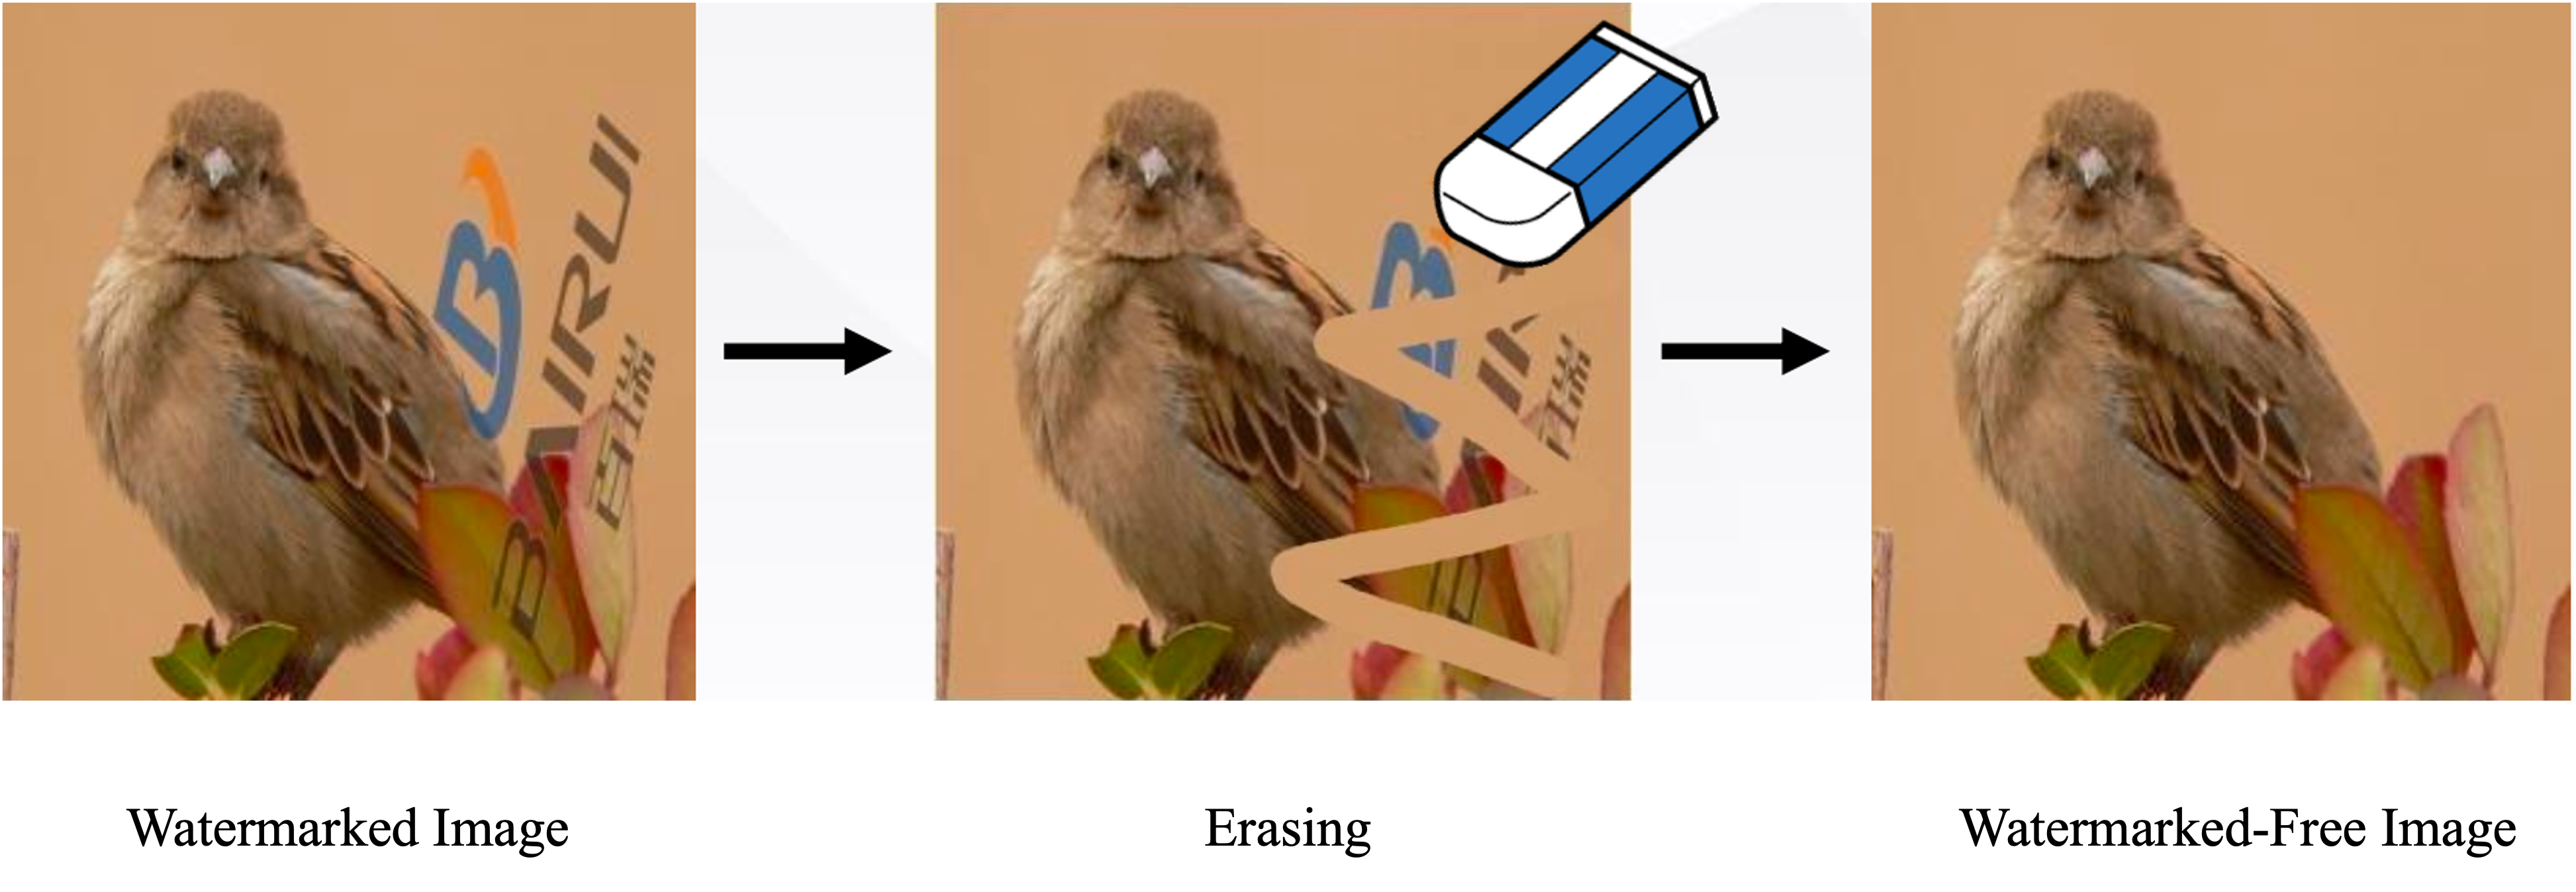
\includegraphics[width=\linewidth]{01.png}
	\vspace{-1cm}
	\captionof{figure}{\small 嵌入水印的载体图像及水印去除的恢复图像}
	\label{fig:01}
	\end{center}  \vspace{3mm}
	\end{minipage}
}]

\section{简介}
\label{sec:introduction}

随着社交媒体的激增,图像和视频成为最流行的记录和传递信息的载体。近年来,数字水印技术已被广泛用于防止图像、视频等多媒体内容非法复制或盗窃的有效解决方案。根据嵌入载体图像中水印数据的可见性将水印技术分为可见和不可见两类。通常,不可见水印适用于作为大多数形式的数字内容知识产权保护机制。除非使用特定的水印提取技术,否则用户无法从视觉感知上区分不可见水印内容和原始载体内容。通过检查可疑内容中是否存在水印,以被动的方式保护内容提供者或作者的版权。而可见水印用于保护必须出于某些目的而发布的数字图像或视频,例如在远程学习网站或数字图书馆中使用的内容,且非法复制是被禁止的。可见水印以更积极主动的方式保护知识产权——可见水印内容通常包含可识别但不显眼的版权图案,用于指示知识产权所有者的身份。除非水印图案能够在不破坏所保护内容的视觉质量的情况下被完全去除,否则没有人可以直接使用带有可见水印的数据。因此,为了满足用户高质量的视觉观感需求,有效的水印去除的图像视频修复技术是必要的。同时,可见水印的嵌入也可能会导致模型学习到错误的特征,进而抑制下游任务的准确性,故需要通过对图像和视频中的水印进行去除和修复以实现更高精度的识别或定位。除此以外,水印去除也可以看作是对水印嵌入图像的一种攻击,而研究如何有效地去除可见水印也为发明更鲁棒的水印嵌入技术提供了线索。

可见水印的嵌入一般是通过将水印图案与载体图像通过 $\alpha$ 混合叠加在一起的。一张带水印的图像$X$通常是通过将水印$W$叠加到载体图像$Y$上获得的。在水印嵌入区域中,水印像素$X(p)$和无水印像素$Y(p)$之间的关系可以表示为:

\begin{equation}
X(p)=\alpha(p) W(p)+(1-\alpha(p)) Y(p)
\end{equation}

其中,$p=(i,j)$ 表示图像中的像素位置,$\alpha(p)$ 是空间变化的不透明度,即图像处理中使用的$\alpha$通道。最常用的水印是半透明的,以保持载体图像内容部分可见,这意味着对于所有像素,$\alpha(p)$的取值范围在$[0, 1]$之间。如果$\alpha(p)$在所有位置上都等于1,那么X就变成了$W$;而如果$\alpha(p)$在所有位置上都等于0,那么$X$就等于$Y$。

水印去除旨在从带水印的图像X中获取无水印的图像$Y$。在给定$W$和$\alpha$的条件下,可以通过逐像素的反向进行操作,简单地逆向合成水印图像的过程

\begin{equation}
Y(p)=\frac{X(p)-\alpha(p) W(p)}{1-\alpha(p)}
\end{equation}

而无水印区域在$X$和$Y$之间保持不变。这一想法不仅适用于传统方法,在给定水印嵌入先验信息的条件下,也可以为水印去除的图像视频修复提供用于指导的边信息。
\section{手工特征和强约束先验}
\label{sec:tradition}

\subsection{不同模式水印的攻击方案}

自从水印技术发明以来,研究人员就一直致力于开发去除技术来攻击它们。由于可见水印的多样性,开发鲁棒的可见水印检测和去除方法是一项具有挑战性的任务。更具体地说,可见水印可能由文本、符号、图形等组成,导致从未知和多样化的水印模式中提取有区分性的特征较为困难。此外,不同类型的水印图像中水印的形状、位置、透明度和大小的变化使得在实际情况下难以估计水印嵌入区域。Huang 等~\cite{huang2004attacking}在基于对可见水印及其嵌入特性的基础上,提出了一种只需要少量人工干预的可见水印去除方案。该方案对于完全由细小图案构成的水印,基本的图像恢复(Image Inpainting)技术可以完全去除嵌入的图案。对于更一般的由粗大图案构成的水印,不仅将利用未标记区域的信息,还将利用水印区域内的信息来正确恢复载体图像。尽管所提出的方案不能保证恢复的图像与未标记的原始图像完全相同,但嵌入图案的结构将被严重破坏,并且可以得到一个在感知上令人满意的恢复图像。这一方案的设计,依赖于下述观察:

\begin{itemize}
	\item 由于嵌入的可见水印应该是不显眼的,并且能够保留原始细节,因此水印模式不应包含复杂的纹理或形状结构。事实上,大多数版权模式都是由几种颜色和平坦区域组成的简单的标志或商标。因此,可以合理地假设可行的水印模式是简单的形状和几种固定的颜色,并且普通用户可以轻松选择水印区域的边界。
	\item 嵌入内容中图像细节的可感知性依赖于水印区域内包含的边缘信息的保留。
	\item 用户能够识别水印内容中包含的版权模式主要是因为嵌入模式的形状(轮廓)被保留并且可以与载体内容区分开。如果嵌入的可见水印的轮廓被完全删除或严重扭曲而不引入严重的视觉质量降低,内容所有者将无法再对非法使用者主张其版权。
	\item 可见水印方案的鲁棒性主要在于必须付出大量的人力劳动才能移除水印。因此,一个有效的攻击方案应尽可能少涉及用户干预。但是在攻击过程中,仍然需要某种用户干预,即手动选择水印区域。这是因为目前没有自动识别机制可以正确找出嵌入的水印区域,除非拥有关于水印模式和嵌入参数的特定领域知识。
	\item 为了设计一个通用的攻击机制,只能利用水印内容中的信息。也就是说,在一个带水印的图像中,只有未标记区域中的像素和水印区域内的剩余信息可以在水印去除过程中利用。其他信息,例如嵌入参数或水印图像的实际强度,被假定为未知,因为攻击者只能获取到嵌入的内容。
\end{itemize}

\begin{figure}[!htbp]
	\centering
	
\includegraphics[width=\columnwidth]{02.png}
	\caption{可见水印示例}
\end{figure}

对于图案非常简单的可见水印通常由标识受保护数字内容版权的文本、商标或符号组成,并且这些图案的宽度(即线条粗读)通常是有限的。在攻击者选择被嵌入水印图案占据的区域之后,水印攻击问题就类似于图像恢复问题。所选区域可以被视为待恢复的区域,其相应的细节被假设为未知。显然,选定区域与周围未改变区域之间存在很高的相关性;因此,我们可以根据周围未改变区域中包含的强度信息来重新填充这些水印区域。最直接的攻击方法是使用一定大小窗口内所有附近未标记像素的平均强度值来重建水印像素值。水印区域可以逐层缩小,恢复的像素值可用于恢复下一个内部像素。最终,将获得一个近似的水印区域版本。当恢复区域位于原始图像的平坦区域内时,这种平均技术可以获得良好的感知质量,但当水印嵌入在跨越物体边界或包含复杂纹理的位置时,将会出现明显的模糊或伪影,如图 \ref{fig:03}所示。

\begin{figure}[!htbp]
	\centering
	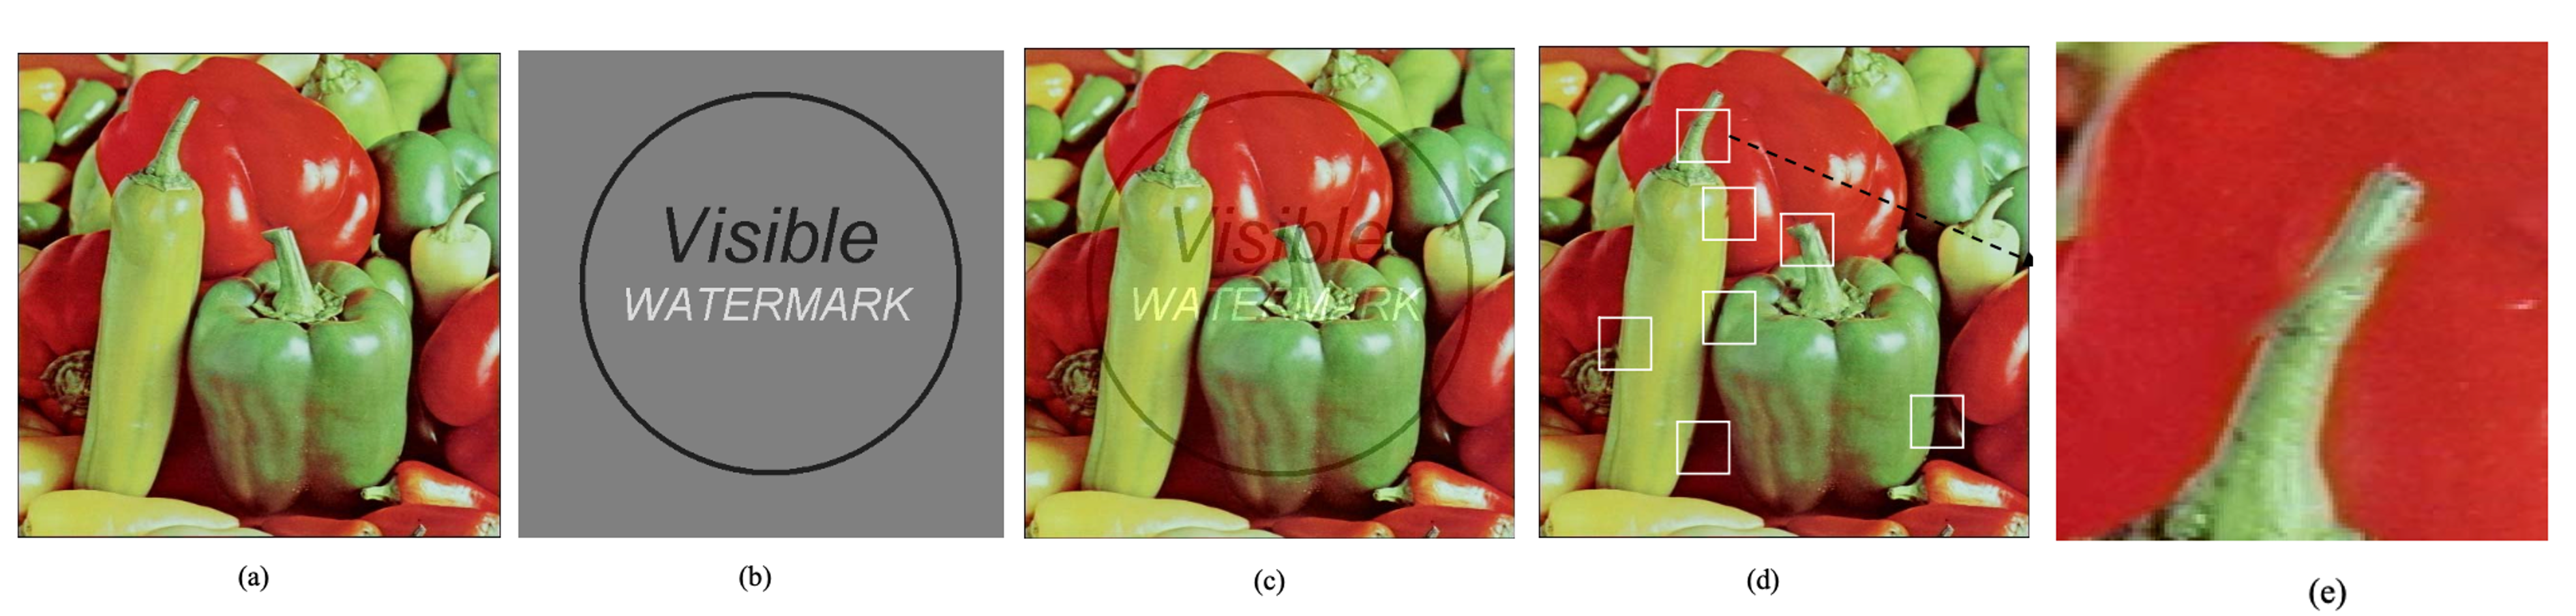
\includegraphics[width=\columnwidth]{03.png}
	\caption{基于平均强度值的恢复结果}
	\label{fig:03}
\end{figure}

图像修复(Image inpainting)技术以不可检测的形式对图像进行修改,以便恢复损坏的区域或移除不需要的对象,其基本思路是来自周围区域的信息被传播到所选区域中。基于修复技术的攻击相比于平均攻击更有效的原因在于前者延长了逼近边缘达到待修复区域边界的过程。整个修复过程可以通过迭代过程实现。

\begin{figure}[!htbp]
	\centering
	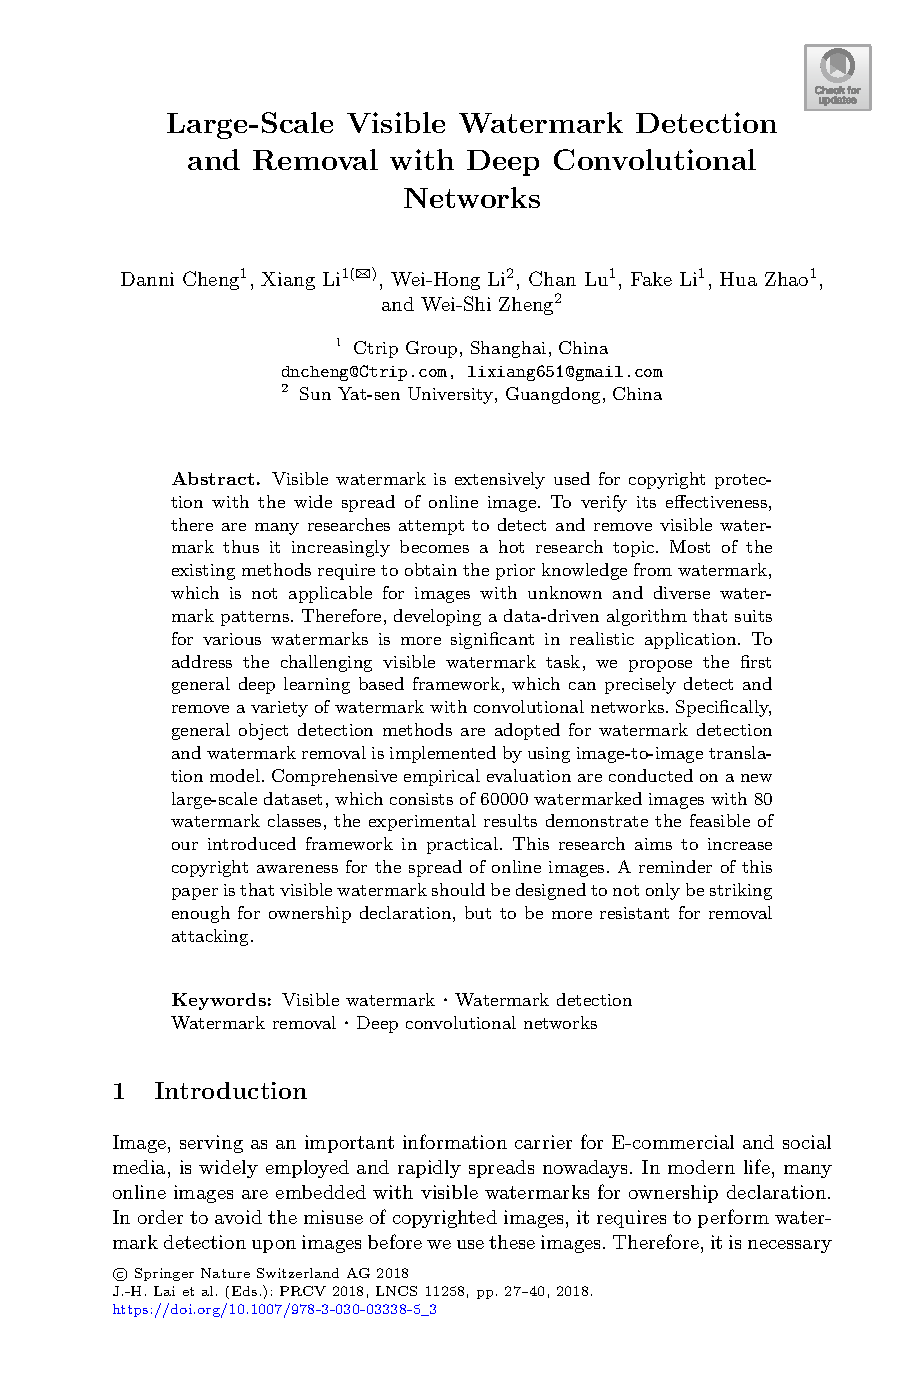
\includegraphics[width=\columnwidth]{04.png}
	\caption{基于图像修复的恢复结果}
	\label{fig:04}
\end{figure}

图像修复技术可以成功去除由细线组成的可见水印模式。然而,更常见的水印可能采用由粗线组成的图案。例如,一家公司可能会在其商标或标志中使用粗体或强调的文字来吸引消费者的注意。如果直接在可见水印方案中采用这种类型的模式,水印区域将占据主图像的相当大部分。因此,仅考虑未标记信息的简单图像恢复技术效果不佳。如图\ref{fig:05}所示,显然,与内部水印文字对应的重新填充区域是不正确的。原因很明显:由于正在被攻击的线现在较粗,远离水印区域边界的像素与已知像素的相关性较低,并且仅使用未标记信息无法正确预测它们。在恢复水印区域中心的像素时,来自不同强度的周围区域的信息将相互干扰。

\begin{figure}[!htbp]
	\centering
	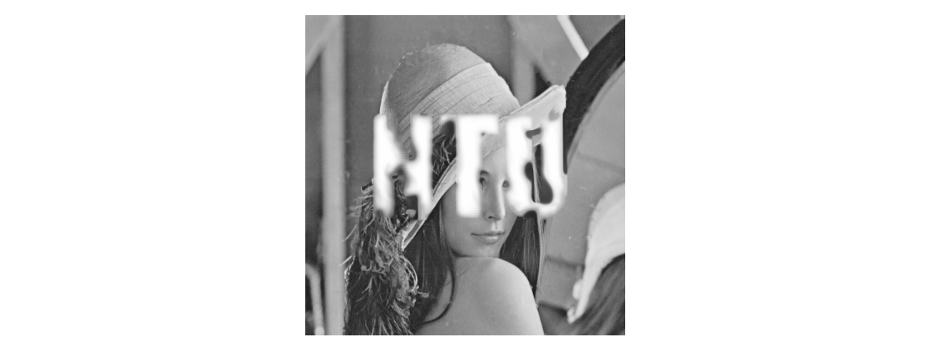
\includegraphics[width=\columnwidth]{05.png}
	\caption{粗线水印图案的恢复结果}
	\label{fig:05}
\end{figure}

如前所述,水印在嵌入之后应该保留原始图像的边缘信息。否则,将无法满足图像细节可感知性的要求。一般来说,水印区域和未标记区域可以很容易地分类为边缘区域和平坦区域。此外,由于在攻击开始时用户可以轻松获得水印模式的形状信息,由水印边界分割的平坦区域(即由标记和未标记区域组成的平坦区域)可以被快速识别和提取出来。由于平坦区域内的像素具有相似的强度值,可以根据同一平坦区域内的未标记信息轻松地填充平坦区域内的标记区域。

\begin{figure}[!htbp]
	\centering
	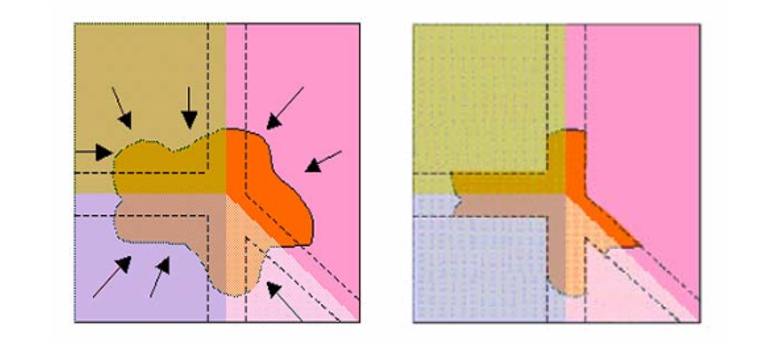
\includegraphics[width=\columnwidth]{06.png}
	\caption{平坦区域恢复原理示意图}
	\label{fig:06}
\end{figure}

如图\ref{fig:07}所示,到目前为止,原始水印图案的形状和结构已经被严重扭曲,大部分重新填充的区域呈现出感知上正确的颜色。尽管某些水印区域保持不变,但嵌入的水印图案已不再可识别。也就是说,嵌入的版权图案现在变得无效。

\begin{figure}[!htbp]
	\centering
	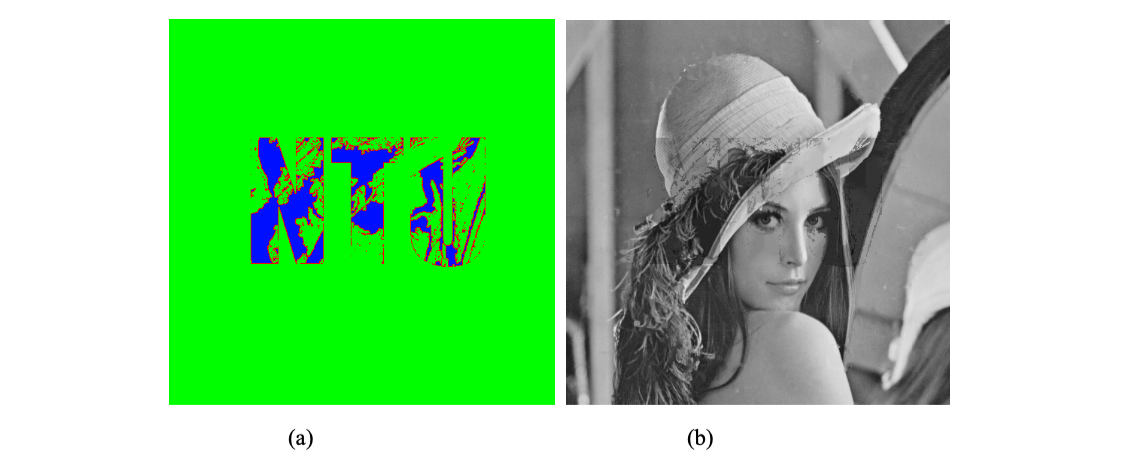
\includegraphics[width=\columnwidth]{07.png}
	\caption{平坦区域恢复结果}
	\label{fig:07}
\end{figure}

尽管可以通过探索剩余的边缘信息来识别和分类所有平坦区域,但只有包含未标记像素的区域才能正确填充。完全位于水印区域内的平坦区域无法获得任何有用的信息,因此只能保持不变。剩下的水印区域现在由完全包含的平坦区域和粗线条水印模式对应区域内的边缘区域组成。

由于使用了水印区域和未标记区域中的所有可用信息,剩余的区域只能通过近似预测来恢复。通过保持边缘和其周围平坦区域之间的强度差异来自动恢复边缘区域,这些区域可能在之前的步骤中原本未被标记或已恢复。边缘的强度根据周围恢复的平坦区域中强度增加或减少的平均量进行调整。尽管水印算法使用的实际颜色变化模型可能非常复杂,并且在攻击过程中不可用,但恢复的边缘区域在感知上是不显眼的。这个结果是合理的,因为边缘区域与周围平坦区域之间的对比仍然保留。虽然无法精确恢复边缘区域的实际强度,但感知的语义得到了很好的保留。实际上,即使在嵌入可见水印之后,由于要求保留原始图像的细节,语义始终存在。

\begin{figure}[!htbp]
	\centering
	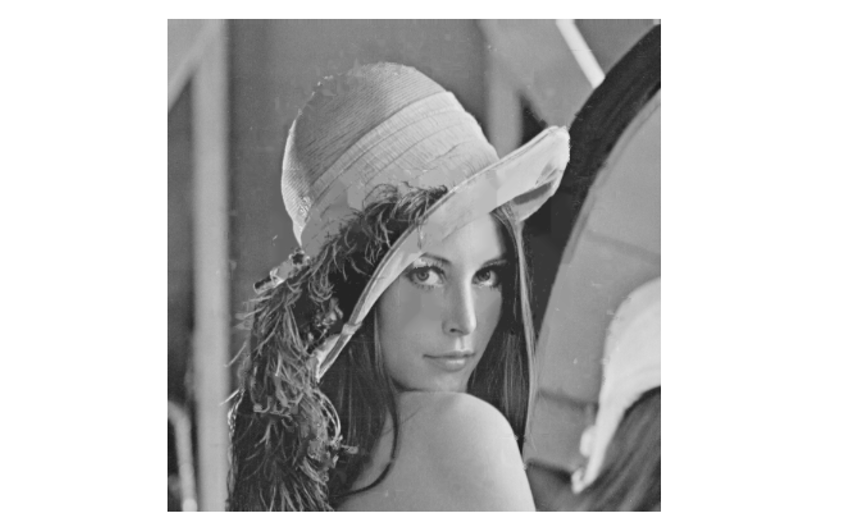
\includegraphics[width=\columnwidth]{08.png}
	\caption{基于可见水印攻击算法的恢复结果}
	\label{fig:08}
\end{figure}

最后,为了恢复完全包含的平坦区域,再次采用了应用于水印边缘区域的相同算法。唯一的区别是根据周围恢复的边缘中出现的像素强度变化量来调整像素强度。由于保留了水印边缘和水印内完全包含的平坦区域之间的差异,恢复的图像在感知上是不显眼的。除了使用预测外,可以统一和手动地调整完全包含的平坦区域的强度值,因为剩余区域非常小且分布稀疏。尽管用户干预是不可避免的,以决定适当的统一强度变化量,但攻击者的工作很简单,因为在提出的攻击的先前阶段已经自动生成了剩余区域的掩码。攻击者可以轻松地迭代地决定适当的强度变化量。

\begin{figure*}[!htbp]
	\centering
	\includegraphics[width=\linewidth]{09.png}
	\caption{基于可见水印攻击算法的恢复结果}
	\label{fig:09}
\end{figure*}

完整的算法流程如下:

\begin{enumerate}
	\item[(i)] 通过用户干预获得表示水印区域的掩码$\mathrm{M}$值;
	\item[(ii)] 应用数学形态学运算操作将$M$分成$\mathrm{M}_{\text {thin }}$和$\mathrm{M}_{\text {thick,}}$两部分,分别表示细线组成的图案和粗线组成的图案相对应的区域;
	\item[(iii)] 通过修复攻击来恢复属于$\mathrm{M}_{\text {thin }}$的区域;
	\item[(iv)] 对整个水印图像的区域使用边缘检测器,并基于阈值  $\mathrm{T}_{\text {edge. }}$将$\mathrm{M}_{\text {thick }}$  分为边缘($\mathrm{M}_{\text {thick }}^{\mathrm{E}}$)和平坦区域($\mathrm{M}_{\text {thick }}^{\mathrm{F}}$);
	\item[(v)] 基于$\mathrm{M}$和$\mathrm{M}_{\text {thick }}^{\mathrm{F}}$,恢复具有未改变近邻的平坦水印区域($\mathrm{M}^{\mathrm{F}-\mathrm{D}}_{thick}$);
	\item[(vi)] Attack remaining edged watermarked areas $\left(\mathrm{M}_{\text {thick }}^{\mathrm{E}}\right)$ by approximated prediction basing on intensity adaptation information of nearby pixels in $\mathrm{M}^{\mathrm{F}-\mathrm{D}}$ thick, obtained in step (v).
	\item[(vii)] 通过基于在步骤(vi)中恢复的$\mathrm{M}_{\text {thick }}^{\mathrm{E}}$的附近像素的强度调整信息的近似预测,攻击完全包含在水印内的平坦区域($\mathrm{m}^{\mathrm{f}-\mathrm{c}}$);	
	\item[(viii)] 如果恢复的图像质量不令人满意,则设置新的阈值$T_{\text {edge }}$,返回步骤(iv),继续迭代。

\end{enumerate}

基于提高可见水印方案鲁棒性的目标,作者提出以下建议:
\begin{enumerate}
	\item[(i)] 在嵌入水印时,应将载体图像的边缘信息视为水印嵌入的参数,因为在平坦区域恢复之后,剩余水印图案的形状极大受到载体图像的边缘结构的影响。例如,将可见水印嵌入到包含高度纹理图案或渐变色分布的区域,无疑会增加水印去除的难度。
	\item[(ii)] 充分增加嵌入图案的形状或纹理复杂性将增加正确选择水印区域的难度。例如,带有抗锯齿边界的水印图案在其精确轮廓之外具有模糊区域。这些模糊区域的强度值与周围透明像素的强度值只有微小的差异,在进行水印选择时可能很容易被忽视。这些区域在经过水印攻击技术后可能介于带水印和未带水印强度值之间,呈现出部分可识别的嵌入图案,需要用户进一步干预。
	\item[(iii)] 为了检测图像是否曾经嵌入可见水印图案,应采用不可见易碎水印(invisible fragile watermarks)技术,即可以使用易碎水印来保护可见嵌入图像的完整性。因此,通过添加不可见易碎水印提供的双重保险,可增强可见水印技术的安全性。当然,在这种情况下,“可见水印方案是否安全?”的问题现在转变为易碎水印的安全问题。
\end{enumerate}

\subsection{强约束的图像组水印去除}

\begin{figure}[!htbp]
	\centering
	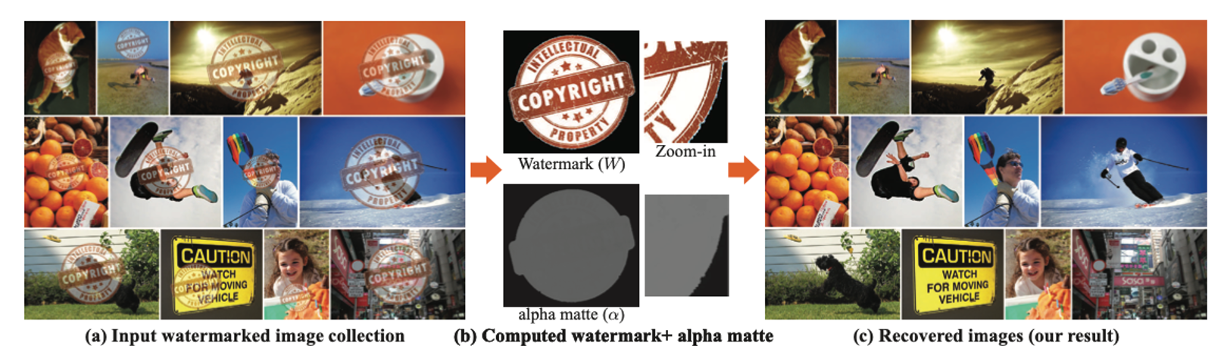
\includegraphics[width=\linewidth]{10.png}
	\caption{水印以一致的方式添加到图像集合}
	\label{fig:10}
\end{figure}

可见水印通常包含复杂的结构,如细线和阴影,以增加其难以去除的程度。因此,在没有用户监督或先验信息的情况下,从单张图像中去除水印是一项极其困难的任务。然而,迄今为止,人们忽视了水印以一致的方式添加到许多图像中的事实。例如,内容存储供应商(Stock Content Marketplace)通常在网络上的数百万张图像预览中添加类似版本的水印。基于这一观察,Dekel 等~\cite{dekel2017effectiveness}将图像集合中的水印去除问题形式化为广义的多图像抠图问题,其目标是利用许多观察到的示例来估计“前景”(水印)图像和 $\alpha$ 蒙版,以及“背景”(原始)图像。具体而言,首先利用数据的冗余性提取整个图像集合中一致的图像结构,以获得抠图水印的初始估计,并在所有图像中检测水印区域。然后,通过解决一个优化问题,将抠图水印分离为图像和 $\alpha$ 蒙版组件,同时重建一部分背景图像。

如图\ref{fig:11}所示,第一步是确定图像集合中哪些图像结构属于公共水印,并在所有图像中对它们进行检测。这是一个先有鸡还是先有蛋的问题,因为估计水印需要知道图像中的水印区域,反之亦然。本文通过联合估计抠图水印和在所有图像中检测水印来解决这个问题。具体而言,在以下估计和检测步骤之间进行迭代。

\begin{figure*}[!htbp]
	\centering
	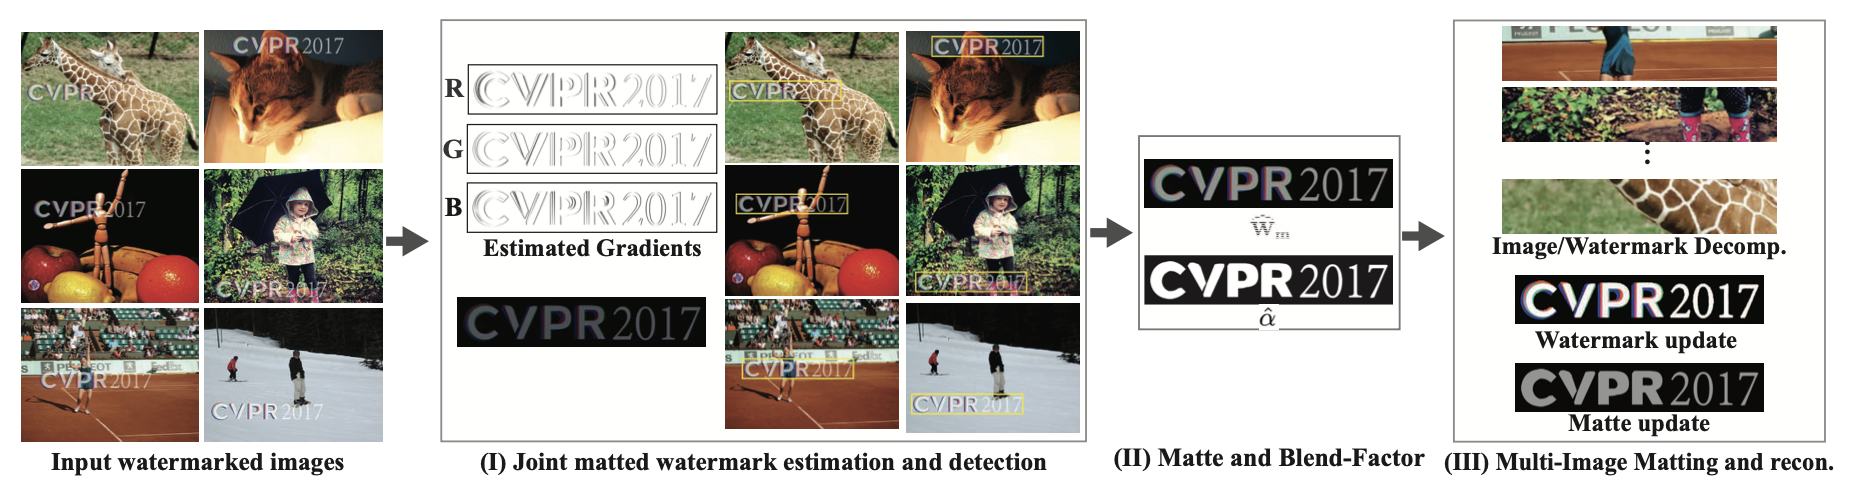
\includegraphics[width=\linewidth]{11.png}
	\caption{自动水印提取流程示意图}
	\label{fig:11}
\end{figure*}


\noindent\textbf{水印估计}:给定当前图像中水印区域的估计,通过观察整个图像集合中一致的图像梯度来确定哪些图像结构属于公共水印。具体而言,在每个像素位置$p$的$x$和$y$方向计算水印图像梯度的中值:

\begin{equation}
\nabla \widehat{W}_m(p)=\operatorname{median}_k\left(\nabla J_k(p)\right)
\end{equation}

当图像数量$K$增加时,不考虑偏移,其将收敛到真实抠图水印$W_m = \alpha W$的梯度。将$I_k$和$J_k$视为随机变量,并计算期望$E [\nabla J_k]$,有:

\begin{equation}
\begin{aligned}
E\left[\nabla J_k\right] & =E\left[\nabla W_m\right]+E\left[\nabla I_k\right]-E\left[\nabla\left(\alpha I_k\right)\right] \\
& =\nabla W_m+E\left[\nabla I_k\right]-\nabla \alpha E\left[I_k\right]-\alpha E\left[\nabla I_k\right] \\
& =\nabla W_m-\nabla \alpha E\left[I_k\right]
\end{aligned}
\end{equation}

其中第二个等式来自于乘法的导数。第三个等式基于自然图像梯度的已知特性, 即在多 图像中具有相同像素位置的强梯度的可能性很小。因此, $\mathrm{E}[\nabla \mathrm{I_k}] \approx 0$ 。这意味着 $\mathrm{E}[\nabla \mathrm{J_k}]$ 近 以于抠图水印 $\mathrm{W_m}$ 的梯度, 除了 $\nabla \alpha \neq 0$ 的像素。在这些像素处, 梯度被 $\nabla \alpha \cdot \mathrm{E}[\mathrm{I_k}]$ 偏移。通过 十算 $\nabla \mathrm{W_m}(\mathrm{p})$ 的幅值并获取其边缘图像的边界框 (使用阈值 0.4 的 Canny 算法) 来裁剪 $\nabla \mathrm{W_m}$ 以去除边界区域。使用泊松重建算法可以获得初始的抠图水印 $\widehat{W}_m \approx W_m$ (经过平移校正)。

\noindent\textbf{水印检测}:给定当前的梯度估计 $\nabla \mathrm{W_m}$, 使用常用于目标检测和识别中的模板匹配的 Chamfer 距离来检测每个图像中的水印。具体而言, 对于给定的水印图像, 使用 Canny 边缘 检测器生成详细的边缘图像, 并计算其欧氏距离变换, 然后将其与 $\nabla \mathrm{W_m}$ (水平和垂直翻转) 进行卷积, 以得到每个像素到最近边缘的 Chamfer 距离。最后, 水印的位置被确定为距离图 中距离最小的像素。这种检测方法非常稳健, 可以在各种不同水印和不同不透明度水平下提供高检测率。

\begin{figure}[!htbp]
	\centering
	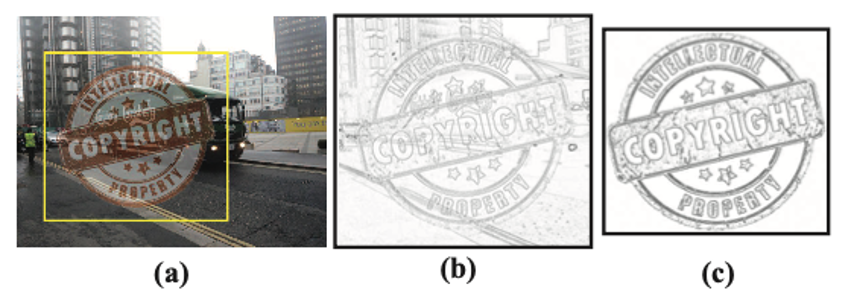
\includegraphics[width=\columnwidth]{12.png}
	\caption{初始的水印估计和检测}
	\label{fig:12}
\end{figure}

对于初始化联合估计,如果图像中水印的相对位置是固定的(正如在网络上观察到的任何图像集合的情况),通过将图像相对于它们的中心进行注册并运行步骤I来获得水印梯度$\nabla \mathrm{W_m}$的初始估计。如果水印位置不固定,只需要用户在其中一张图像周围标记一个粗略的边界框。然后,将给定边界框内的梯度作为水印梯度的初始估计。在步骤I和步骤II之间迭代2-3次足以获得准确的检测结果和可靠的抠图水印估计。

在所有输入图像中进行对齐检测后,目标是解决多图像抠图问题,即将每个图像中观测到的亮度分解为其水印、透明度抠图和原始图像组成部分。通过对下列目标进行迭代优化,即可获得嵌入的水印图案和$\alpha$等先验,并进而用于其他图像的水印去除和恢复。

\begin{equation}
\begin{aligned}
& \underset{W, \alpha,\left\{I_k\right\}}{\arg \min } \sum_k\left(E_{\text {data }}\left(W, \alpha, I_k\right)+\lambda_I E_{\mathrm{reg}}\left(\nabla I_k\right)\right) \\
& \quad+\lambda_w E_{\mathrm{reg}}(\nabla W)+\lambda_\alpha E_{\mathrm{reg}}(\nabla \alpha)+\beta E_f(\nabla(\alpha W))
\end{aligned}
\end{equation}

\begin{equation}
E_{\text {data }}\left(I_k, W, \alpha\right)=\sum_p \Psi\left(\left|\alpha W+(1-\alpha) I_k-J_k\right|^2\right)
\end{equation}

\begin{equation}
E_{\mathrm{reg}}(\nabla I)=\sum_p \Psi\left(\left|\alpha_x\right| I_x^2+\left|\alpha_y\right| I_y^2\right)
\end{equation}

\begin{equation}
E_f\left(\nabla W_m\right)=\sum_p \Psi\left(\left\|\nabla W_m-\nabla \widehat{W}_m\right\|^2\right)
\end{equation}

由于此类攻击依赖于图像集合中水印的一致性,一个自然的想法是是否可以通过打破这种一致性来阻止它。因此,本文研究了该攻击对不同类型的不一致性或变化的鲁棒性,这些不一致性或变化有可能在每个图像中嵌入水印时引入。通过实验发现,例如,随机改变水印在整个集合中的位置并不能阻止该攻击检测和去除水印,水印的不透明度或颜色的随机变化也无法阻止。而在嵌入水印过程中对水印进行小的空间变形可以显著降低去除水印后图像的质量,对水印本身几乎没有察觉到的变化。

\begin{figure*}[!htbp]
	\centering
	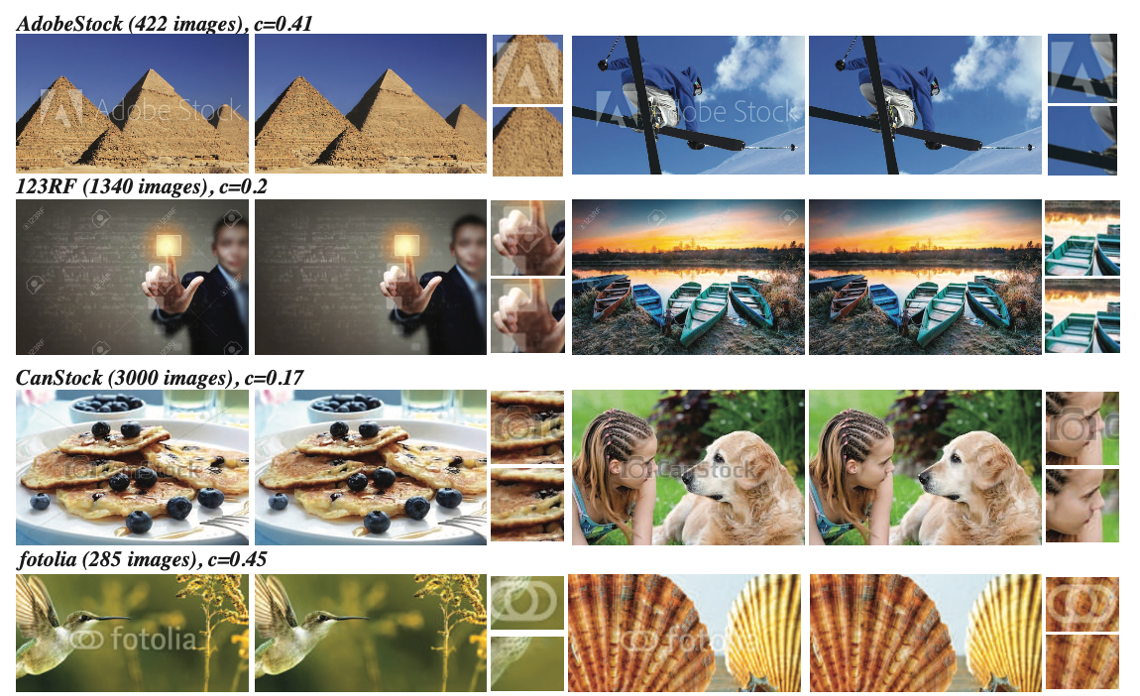
\includegraphics[width=\linewidth]{13.png}
	\caption{水印去除结果}
	\label{fig:13}
\end{figure*}

\subsection{基于镜头思想的视频水印去除算法}

\begin{figure}[!htbp]
	\centering
	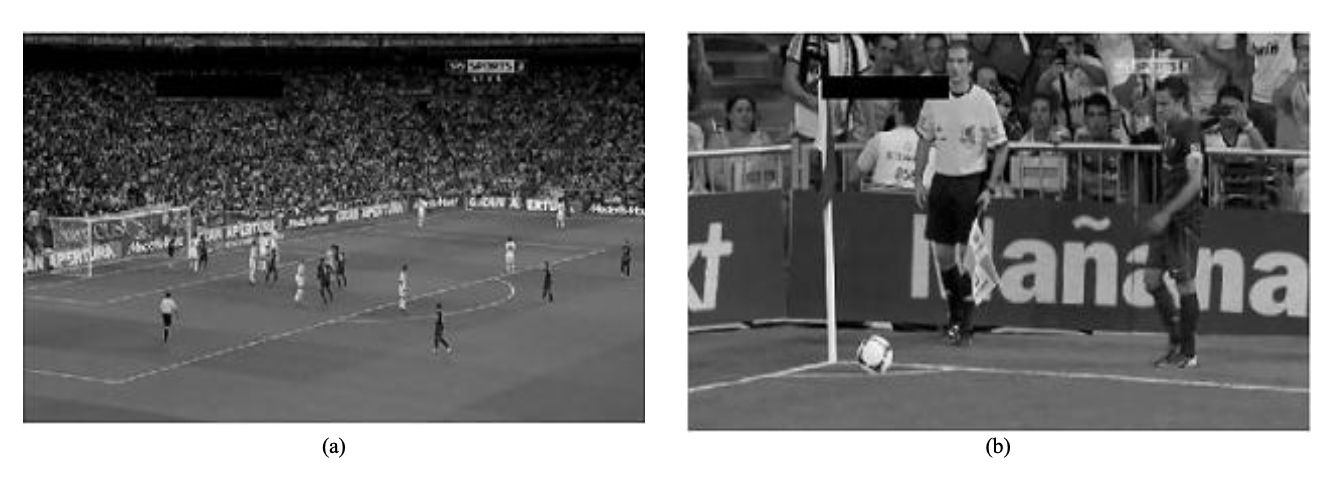
\includegraphics[width=\columnwidth]{14.png}
	\caption{不同视频镜头的两帧}
	\label{fig:14}
\end{figure}

	与多组图像的水印去除不同,视频的水印去除可以依赖于视频的时间连贯性,即在一个帧中被水印遮挡的图像内容在其他帧中是不被遮挡的。通用的视频修复算法为基础的水印去除方法利用下一帧的信息来更好地判断当前图像中缺失的像素值,然而正因为这样的方式不是任意的,因而不能用于在线应用。而且它们具有很高的计算成本,更加抑制了其在真实场景中的应用。为了解决这一问题,Dashti等~\cite{dashti2015video}将视频镜头的思想引入了视频修复算法中。视频镜头是从特定场景中捕捉到的帧序列。如图\ref{fig:14},在足球比赛中,摄像机正在拍摄人群,这是一个视频镜头的一帧,当摄像机改变视角并拍摄裁判员时,这是另一个视频镜头的一帧。每个视频镜头的帧具有结构和统计上的相似性,通常表现出相同类型的纹理。视频镜头是通过计算连续两帧之间的差异的总平均值来定义的。如果这个总平均值足够大,超过了指定的阈值,那么第二帧被检测为新镜头的第一帧。

\begin{figure*}[!htbp]
	\centering
	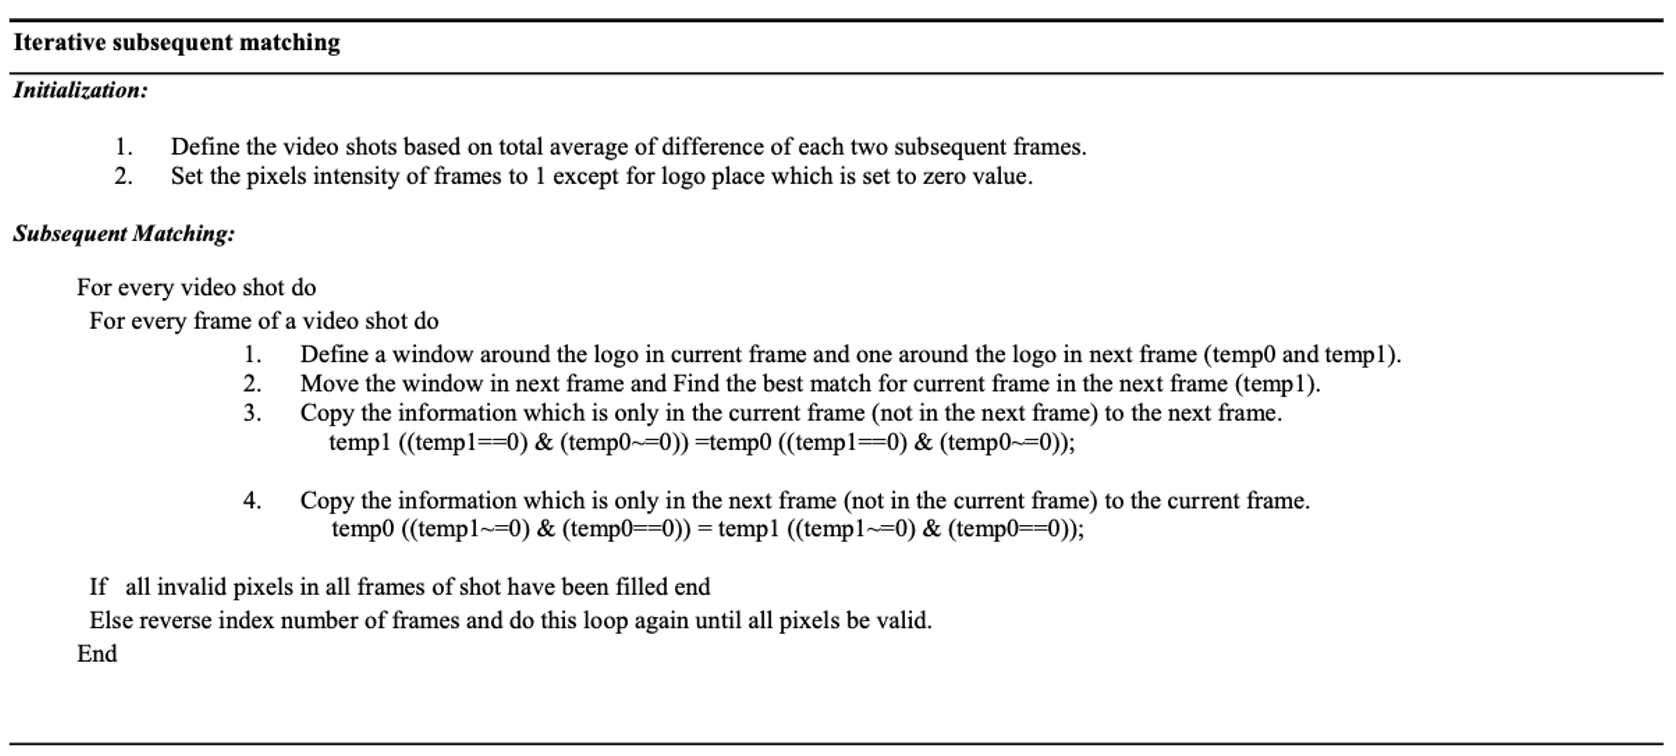
\includegraphics[width=\linewidth]{16.png}
	\label{fig:fig16}
\end{figure*}

	
在定义了视频镜头的概念后,对视频帧缺失像素的查找和填充只需要集中在相同视频镜头的图像帧即可,从而可以有效减少计算开销。为了填充帧中的水印,在水印周围选择一个面积略大于水印的矩形,然后在当前帧和近邻帧中找到与水印周围矩形中的像素值最匹配的位置。每个矩形框都有一些有效像素和一些无效像素,无效像素位于水印位置上。这样做是希望通过周围有效像素的帮助找到无效像素的最佳值,因此,将紧邻帧中的矩形框向上、向下、向右和向左移动几个像素,以找到与当前帧中的矩形框最佳匹配的位置。最佳匹配与当前帧中矩形框包含的有效像素具有最小均方差(LMSE)。

\begin{figure}[!htbp]
	\centering
	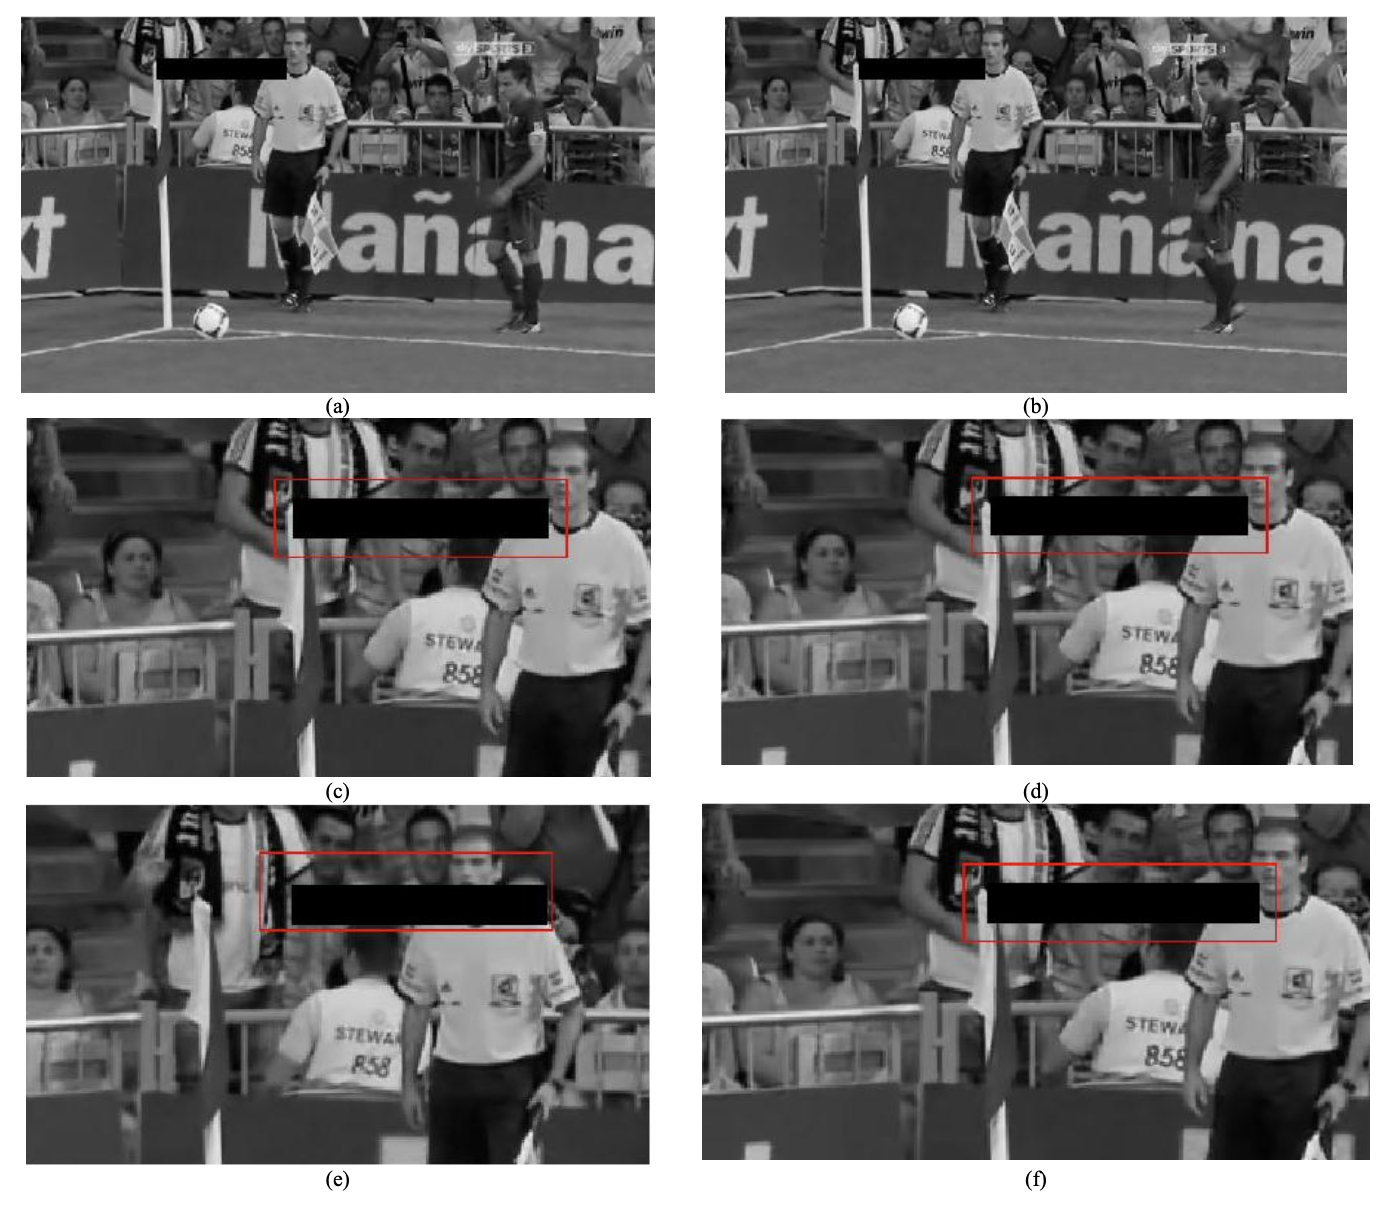
\includegraphics[width=\columnwidth]{15.png}
	\caption{视频水印去除算法样例图}
	\label{fig:15}
\end{figure}

完整的算法流程见上。
\section{基于U-Net和GAN网络的深度学习方法}
\label{sec:gan}


\subsection{大规模可见水印检测和去除数据集}
由于可见水印的多样性,设计鲁棒的可见水印检测和去除方法仍然是一项具有挑战性的任务。具体而言,可见水印可能由文字、符号、图形等组成,导致从未知和多样化的水印模式中提取有区分性的特征较为困难。此外,各种类型的水印图像在嵌入过程中其形状、位置、透明度和大小的变化使得在实际情况下估计水印嵌入区域变得更加困难。现有的可见水印检测和去除工作需要通过从图像中提取手工设计的特征,高度依赖先验知识,抑或是假设水印图像具有相同的水印模式。这种强先验依赖或约束都不适用于在水印可能是未知的、不同图像中的水印更可能是不同的真实场景。而深度卷积网络基于大量图像数据学习特征表示的强大性能,但使得其对未知和多样化水印模式的检测和去除成为可能。

\begin{figure}[!htbp]
	\centering
	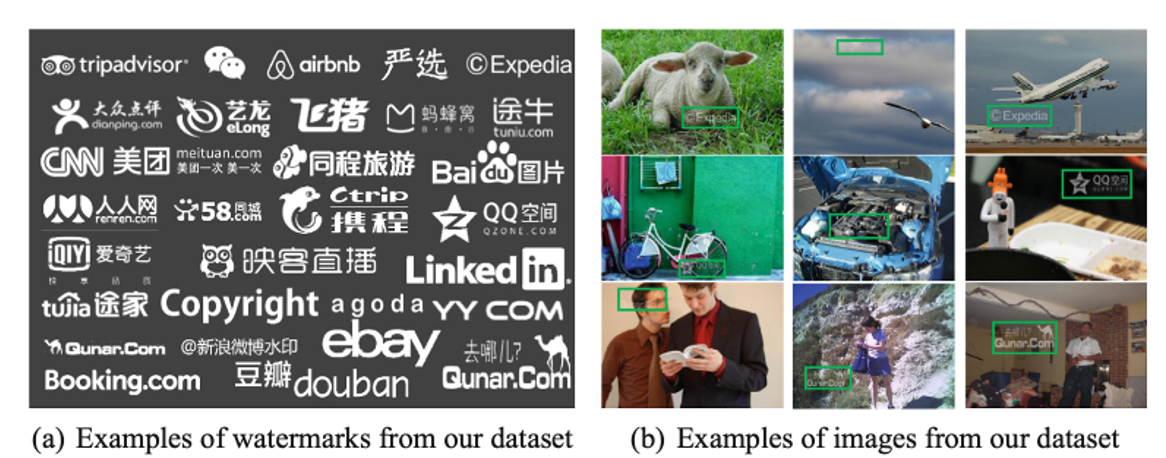
\includegraphics[width=\columnwidth]{17.png}
	\caption{数据集示例图}
	\label{fig:17}
\end{figure}

在水印检测和去除方面,既没有基于深度学习的方法,也缺乏大规模的水印数据集。为了填补这一空白,Cheng 等~\cite{cheng2018large}制作了一个包含60000张由80个水印制成的带水印图像数据集,每个水印有750张图像。具体而言,训练和测试集中使用的原始图像是采用有放回抽样分别从PASCAL VOC2012数据集的训练/验证集和测试集中随机选择的。而80个水印类别采集自知名的电子商务品牌、网站、组织、个人等,涵盖了大量的模式(如包括英文和中文)。此外,不同图像中每个水印的大小、位置和透明度在嵌入时都是随机设置的。该数据集与传统的小规模水印数据集之间的另一个重要区别在于,训练集中的水印不用于构建测试集中的图像。具体而言,在现有的水印数据集中,训练集和测试集中的水印完全相同。这将导致在这种数据集上训练的水印检测器无法很好地检测图像中的未知水印。

\begin{figure*}[!htbp]
	\centering
	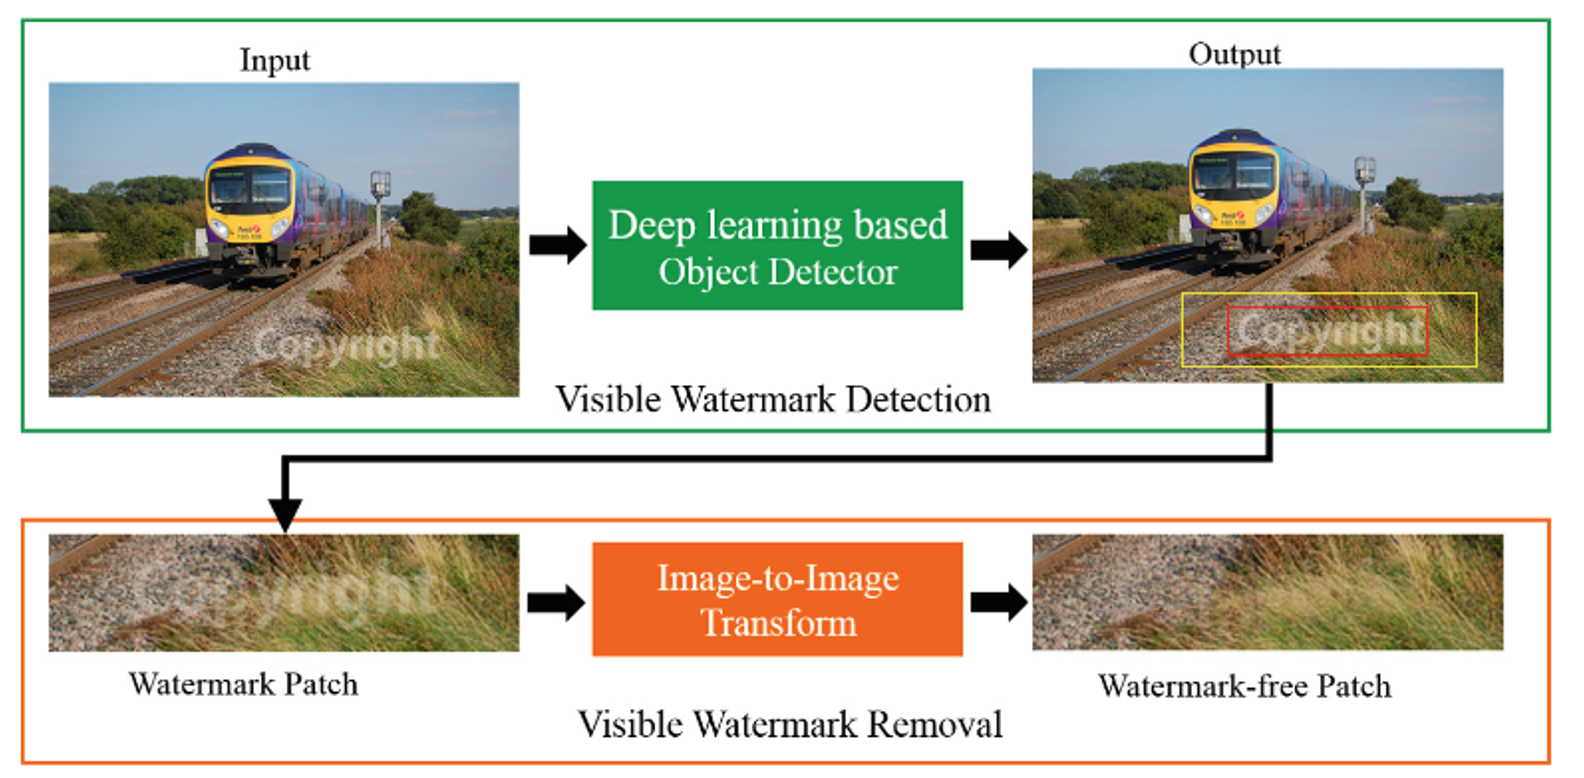
\includegraphics[width=\linewidth]{18.png}
	\caption{可见水印处理框架示意图}
	\label{fig:18}
\end{figure*}

其设计的可见水印处理框架由水印检测和去除两个部分组成。具体而言,采用当前最先进的目标检测器框架作为水印检测网络,如Faster RCNN、YOLO、RetinaNet,并对其进行进一步微调以适应在图像中检测和定位可见水印的任务。一旦图像中的水印被准确检测出来,检测结果可以用于进一步的水印去除。

在去除过程中,将水印去除转化为图像到图像的转换问题,有效地将带水印的像素转换为原始的未标记像素。这一部分包括水印去除网络和损失网络。每个带水印的图像块x被输入到水印去除网络中,以获取估计的无水印图像块˜y。水印去除网络为U-Net架构,其在结构上具有镜像对称性,并且在相应的块之间具有跳跃连接。通过这种方式,使得输入附近的浅层特征与高层特征结合在一起,以便保留输入图像的位置和纹理等低层特征。

\begin{figure}[!htbp]
	\centering
	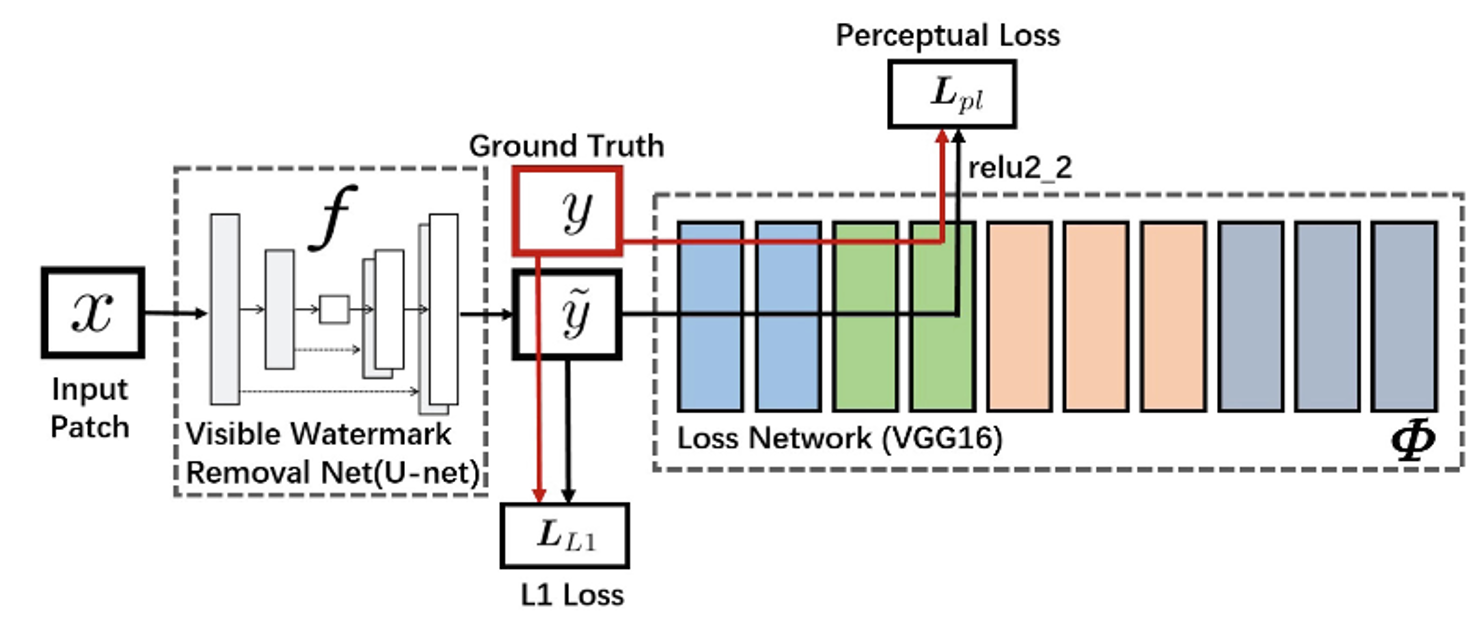
\includegraphics[width=\columnwidth]{19.png}
	\caption{可见水印去除网络架构图}
	\label{fig:19}
\end{figure}

然后,基于真值和估计的图像块计算L1损失和感知损失。与将整个图像进行像素级别的转换不同,该工作侧重于将检测到的区域内的像素恢复到未标记的状态,而水印图像中未标记区域内的像素将保持不变。由于L1损失是基于整个图像逐像素计算的,当每个像素有微小变化且图像在视觉上几乎没有差异时,L1损失会很大。而感知损失被证明在捕捉源图像的语义信息方面是有效的,它依赖于来自卷积层的高级特征,因此,使用感知损失可以得到更加真实的输出结果。

\begin{equation}
\boldsymbol{L}_{\text {whole }}=\boldsymbol{L}_{L 1}+\alpha \boldsymbol{L}_{p l}^{\Phi, \text { relu2 } \_2}
\end{equation}

\begin{equation}
\boldsymbol{L}_{L 1}(x, y)=\|f(x)-y\|_1
\end{equation}

\begin{equation}
\boldsymbol{L}_{p l}^{\Phi, j}(\tilde{y}, y)=\frac{1}{C_i H_i W_i}\left\|\Phi_j(\tilde{y})-\Phi_j(y)\right\|_2^2
\end{equation}

\subsection{更真实的可见水印去除网络}

在传统的可见水印去除方法中,存在两个主要问题。首先,在执行水印去除之前,需要手动标记水印图像中的水印区域和非水印区域。其次,为了有效地去除水印,需要多个具有相同水印的水印图像进行水印去除。Cheng等首次将卷积神经网络引入水印去除任务,有效解决上述两个问题。然而,由于直接训练具有像素级损失的生成器来建模像素映射关系是较为困难的,再加上且他们采用的网络结构简单、损失函数效率低下,他们模型得到的结果并不理想。通过其方法恢复的无水印图像通常仍然包含一些残留的水印痕迹,使得恢复的图像在人类视觉感知上不具备真实感。

\begin{figure}[!htbp]
	\centering
	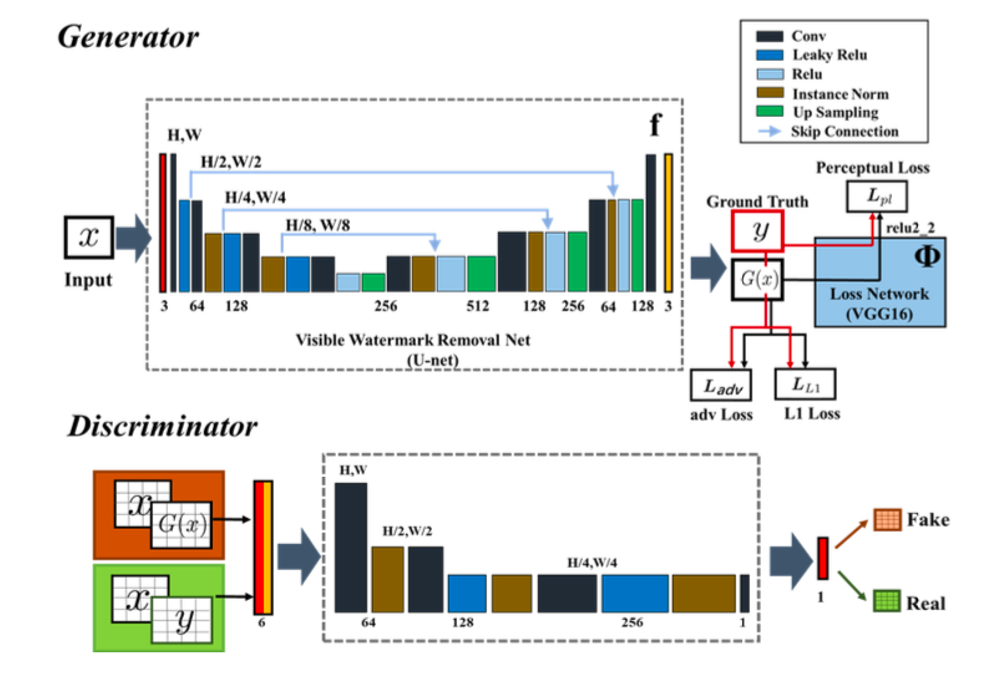
\includegraphics[width=\columnwidth]{20.png}
	\caption{基于条件生成对抗网络的可见水印去除网络架构图}
	\label{fig:20}
\end{figure}


为了使水印去除的结果更具照片般的真实感和可信度(例如,恢复没有任何残留水印的水印区域并使其更具照片般的真实感),Li等~\cite{li2019towards}基于条件生成对抗网络(conditional generative adversarial networks, cGANs)设计了一个照片般真实水印去除的框架。该网络由一个生成器和一个判别器组成,基于U-Net架构的生成器以嵌入了水印的图像作为输入,生成一个逼真的无水印图像。判别器是一个基于图像块的分类器,与常见的GAN判别器将输入映射为表示输入样本“真实”概率的标量不同,它将水印图像和去水印图像的组合映射为特征图,用以表示输入的图像块的“假”或“真”类别概率。由于特征图中的点可以追溯到原始图像中的特定感受野,因此输出矩阵中的每个值表示原始图像中的块是否“真实”的概率。规定输入图像是“真实”的概率为所有图像块为“真实”的概率的平均值。这样做是因为水印图像与原始无水印图像之间的差异仅存在于图像的某些部分。由于水印区域相对于整个图像来说比较小,基于图像块的判别器能够识别两个输入图像的最不同的区域并更加关注最小化这些区域的重建误差。

除此以外,为了使生成器恢复的图像尽可能接近真实的无水印图像,在Cheng等损失函数的基础上引入了新的目标函数,即最终目标函数由 L1 损失、感知损失和基于图像块的对抗损失函数的组成,用于约束生成器的训练。同时,使用一个经过对抗训练的判别器 D 来区分“假”图像和真实图像。

\begin{equation}
\boldsymbol{G}^*=\arg \min _G \max _D \underbrace{\boldsymbol{L}_{\text {adv }}(G, D)}_{\text {adversarial loss }}+\underbrace{\alpha \boldsymbol{L}_{l_1}(G)+\beta \boldsymbol{L}_{p e r}(G)}_{\text {content loss }} .
\end{equation}

\begin{equation}
\boldsymbol{L}_{a d v}(G, D)=\mathbb{E}_{x, y}[\log D(x, y)]+\mathbb{E}_x[\log (1-D(x, G(x)))]
\end{equation}

\begin{figure}[!htbp]
	\centering
	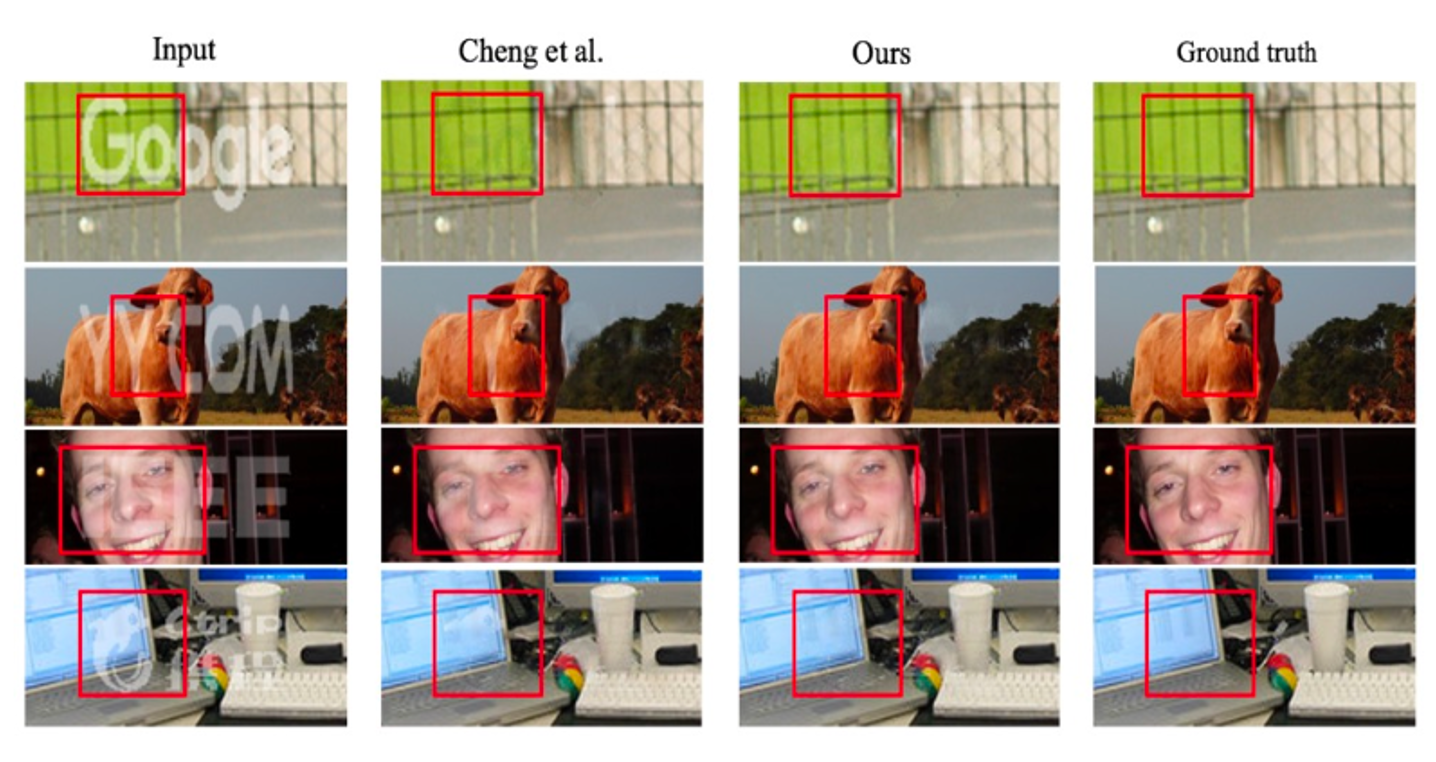
\includegraphics[width=\columnwidth]{21.png}
	\caption{水印去除结果}
	\label{fig:21}
\end{figure}

\subsection{两阶段水印去除架构}

\begin{figure}[!htbp]
	\centering
	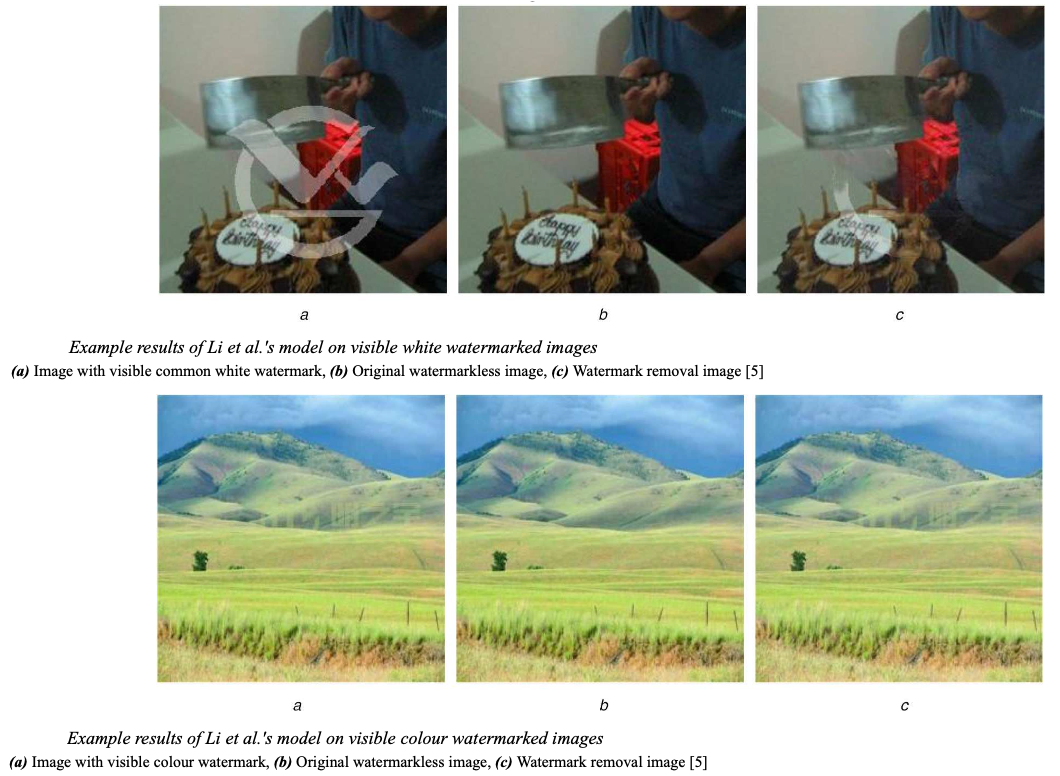
\includegraphics[width=\columnwidth]{22.png}
	\caption{研究动机}
	\label{fig:22}
\end{figure}

Li等在Cheng等定义的损失函数中引入了对抗性损失,使得生成的图像更加逼真。然而,对于白色水印图像,如图1所示,在去除水印后仍然存在残留水印。此外,Li等提出的方法无法去除颜色与背景颜色非常相似的可见水印,如图\ref{fig:22}所示。

基于上述观察,Jiang等~\cite{jiang2020two}提出了一种基于条件生成对抗网络(CGANs)和最小二乘生成对抗网络(least-squares generative adversarial networks, LSGANs)的可见水印去除网络架构。该架构包括水印提取和图像修复两个阶段。首先,第一阶段通过提取网络识别水印特征并提取图像中的水印,该网络主要关注水印图像的水印区域。然后,从水印图像中减去提取的水印,获得初步的去水印图像。最后,第二阶段将初步的去水印图像输入修复网络,以获得更一致和真实的去水印图像。

该工作延续了之前生成对抗网络和U-Net的模型设计,生成器包括提取网络和修复网络两个部分,同样使用两个判别器来区分生成的图像和真实图像。为了使提取的水印更接近真实水印,并使生成的无水印图像更接近真实图像,使用了两个有条件的PatchGAN判别器。与传统的判别器不同,它们可以判断图像中每个区域的真实概率。

\begin{figure*}[!htbp]
	\centering
	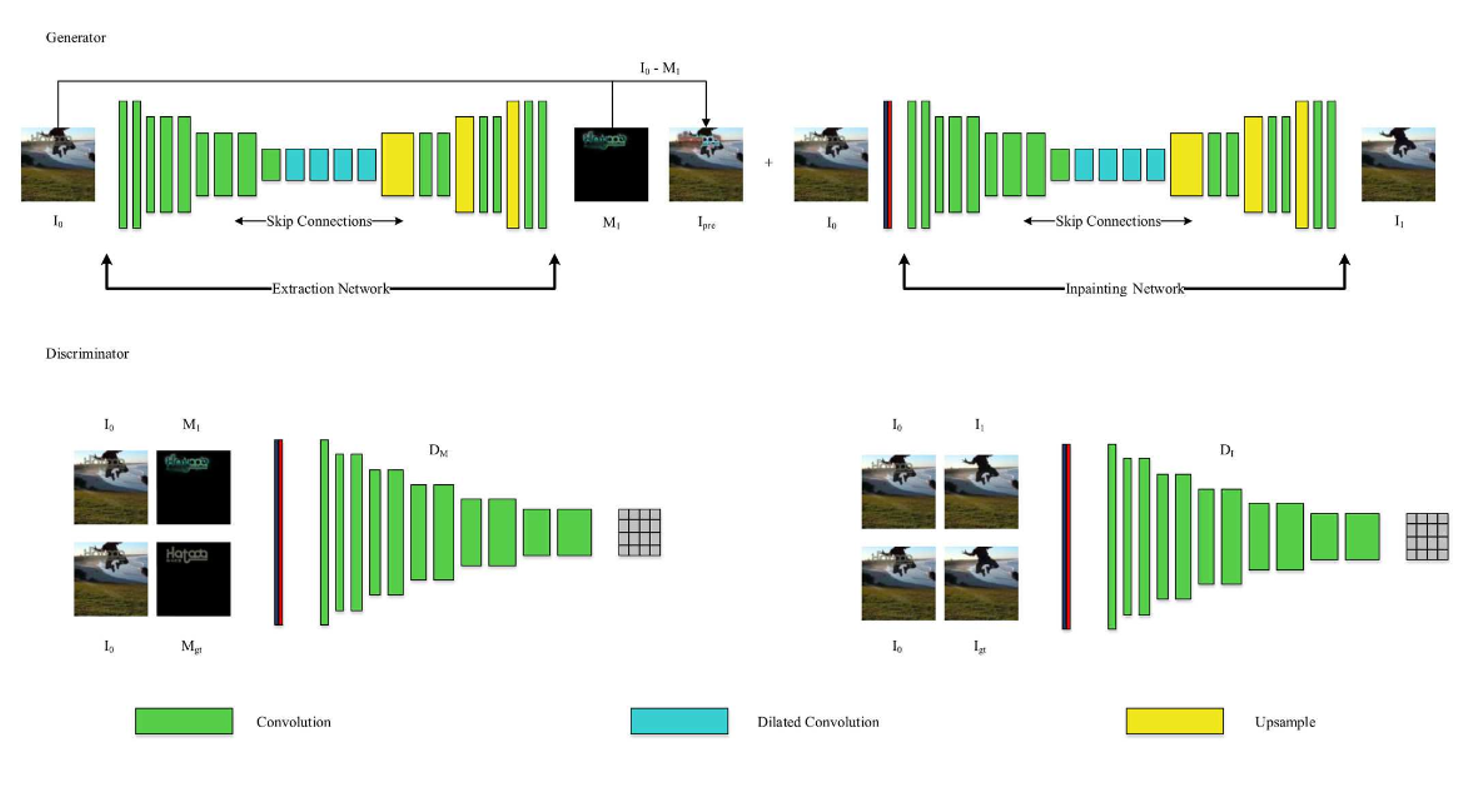
\includegraphics[width=\linewidth]{24.png}
	\caption{基于条件生成对抗网络和最小二乘生成对抗网络的两阶段水印去除框架示意图}
	\label{fig:24}
\end{figure*}


这是首个将图像修复与水印去除相结合的深度学习方法,网络整体更加关注于图像中水印的嵌入区域。该模型通过提取网络可以自动检测水印的位置,因而克服了传统水印去除方法需要手动标记水印区域的缺点。与基于深度学习的方法相比,Cheng等的方法依赖于现有的目标检测方法来检测水印位置,并且其去水印网络具有简单的结构和低效的损失函数。而本文的方法通过端到端训练可以直接为输入的水印图像输出无水印图像,并且由于增加了对抗性损失,输出的无水印图像更加逼真。此外,与Li等的工作相比,该模型更加关注水印区域,从而可以实现更鲁棒和逼真的水印去除。

\begin{figure}[!htbp]
	\centering
	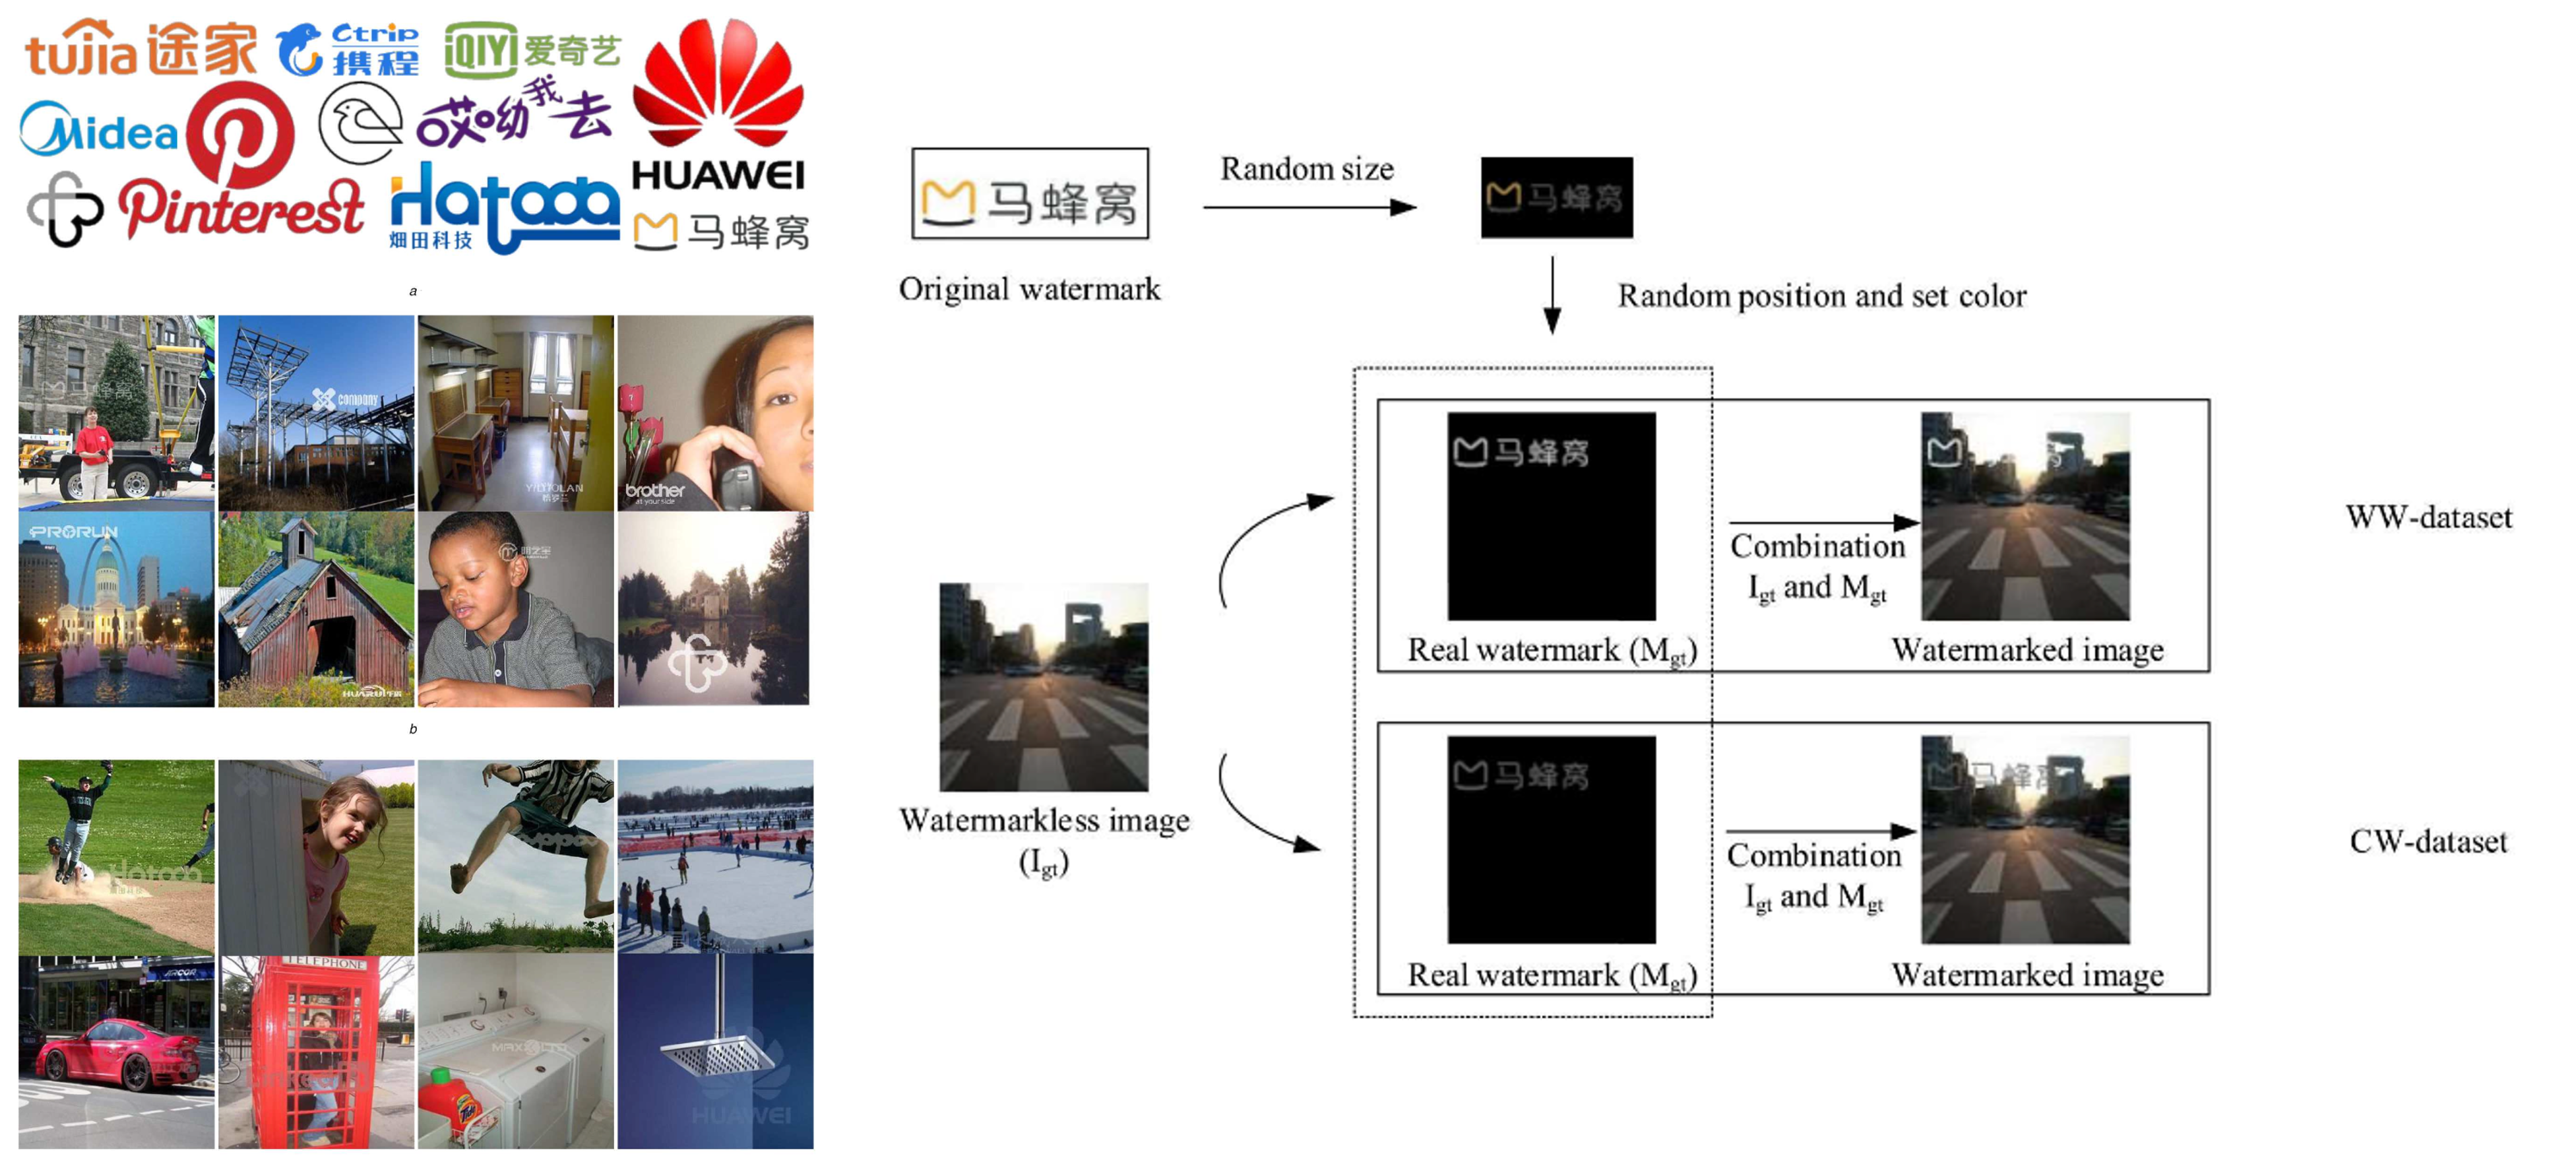
\includegraphics[width=\columnwidth]{23.png}
	\caption{WW数据集和CW数据集}
	\label{fig:23}
\end{figure}

为了评估网络架构的性能,Jiang等建立了两个带有水印的图像数据集——白色水印图像数据集(WW数据集)和彩色水印图像数据集(CW数据集)。两个数据集均包含53,300张带水印的图像,这些图像是由53,300张无水印的图像和100种原始水印生成的。其中53,300张无水印的图像来自于两个公共数据集,即PASCAL VOC2012和places2。而100种原始水印是从互联网上收集而来的品牌、网站等的标识。首先将53,300张无水印的图像平均分成100组(80组作为训练集,20组作为测试集)。然后,每个组中的图像都添加相同的水印,不同组的图像添加不同的水印。两个数据集之间唯一的区别是水印的颜色。如图\ref{fig:fig25}和\ref{fig:26}所示,实验结果表明,所提出的方法具有去除残留水印的能力,并且能够去除接近背景颜色的彩色水印。

\begin{figure}[!htbp]
	\centering
	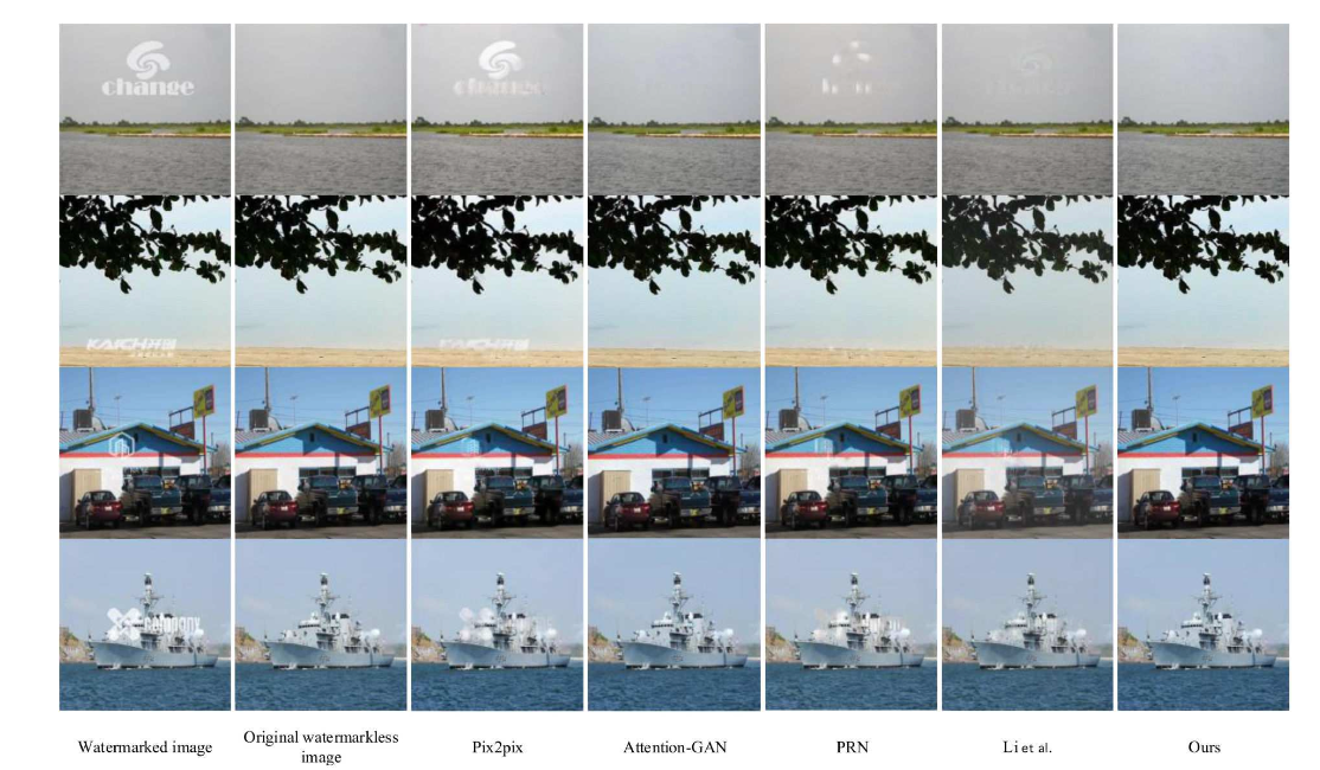
\includegraphics[width=\columnwidth]{25.png}
	\caption{WW数据集水印去除结果}
	\label{fig:25}
\end{figure}

\begin{figure}[!htbp]
	\centering
	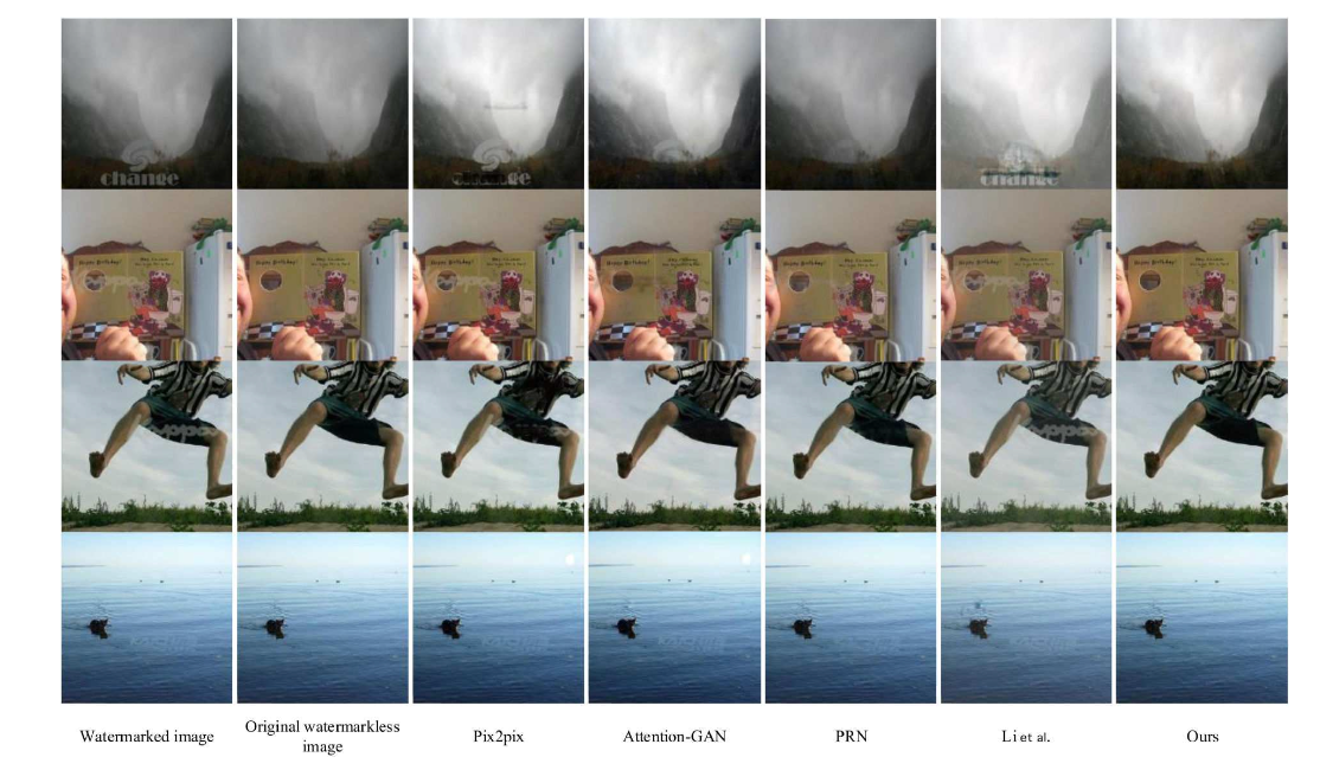
\includegraphics[width=\columnwidth]{26.png}
	\caption{CW数据集水印去除结果}
	\label{fig:26}
\end{figure}

\section{多任务视角下的水印去除}
\label{sec:multitask}

\subsection{“盲”设置下的水印去除}

如前文所述,由于水印图案本身及其在嵌入过程中的复杂多变,没有用户指导或强约束的前提下难以很好地检测和去除它们。但是,在“盲”设定下,这些图案的确切位置、结构和大小是未知的。先前的方法依赖于恢复受损像素的位置信息,即使是深度学习的方法也都依赖于分阶段地对水印嵌入位置进行检测。Hert 等~\cite{hertz2019blind}首次提出了一种完全“盲”的视觉图案去除方法,该网络可以移除在训练过程中未见过的视觉图案,例如从真实世界图片中去除水印。网络首先估计哪些像素包含图案,然后重建潜在图像来分离视觉图案和图像。除了估计二值图案掩模和重建潜在图像之外,该网络还重建了嵌入到载体图像的视觉图案。将输入图像分解为视觉图案和背景图像(载体图像)使网络能够更好地重建图像。

\begin{figure}[!htbp]
	\centering
	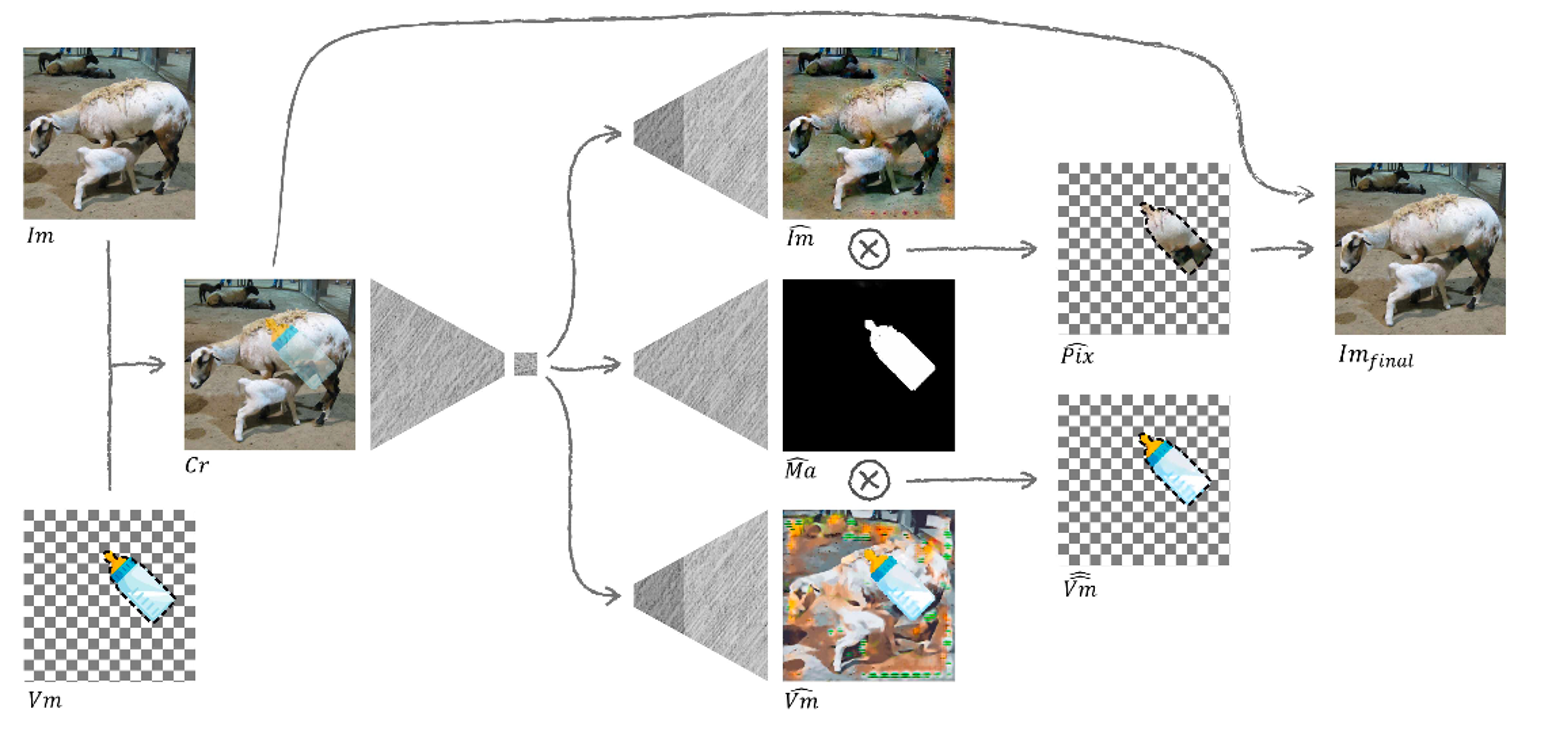
\includegraphics[width=\columnwidth]{27.png}
	\caption{“盲”设定下的多任务水印提取和图像恢复网络架构图}
	\label{fig:27}
\end{figure}

网络通过编码器将嵌入了水印的图像编码为潜在表示,然后通过三个并行的解码器分支进行解码:一个用于估计潜在图像,一个用于估计图案掩模,一个用于估计图案图像。最终的图像通过使用估计的图案掩模从输入图像或重建图像中选择像素来生成。在训练过程中,使用输入图像和视觉图案作为真值来计算损失以优化编码器和解码器网络。

\begin{figure}[!htbp]
	\centering
	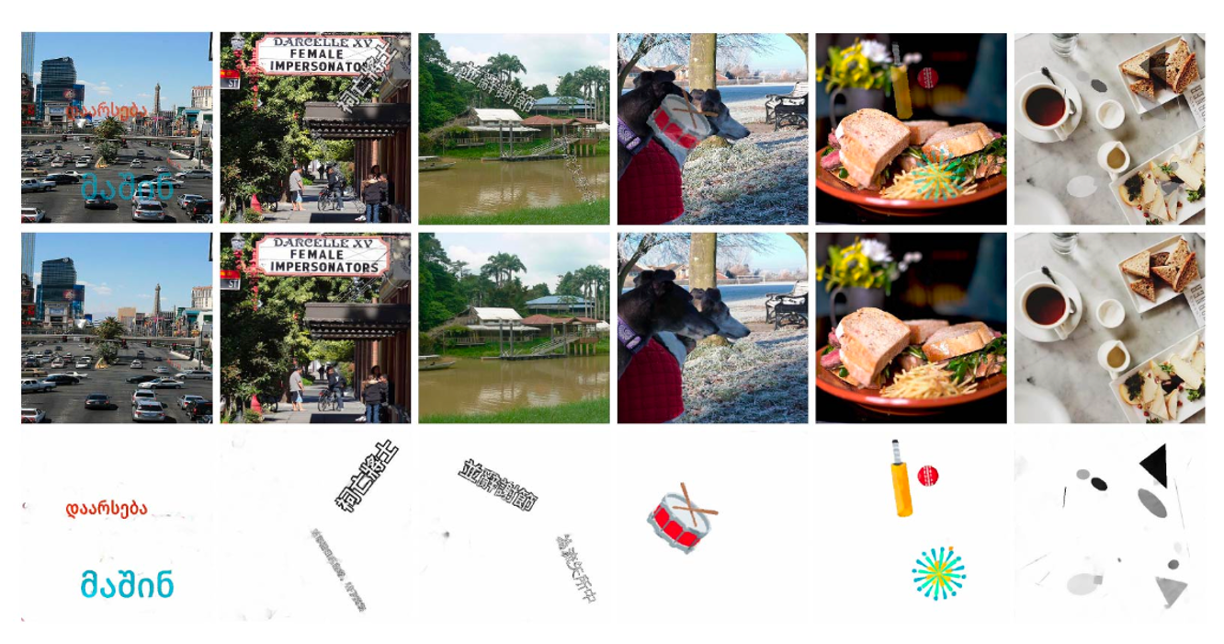
\includegraphics[width=\columnwidth]{28.png}
	\caption{水印提取和图像恢复结果}
	\label{fig:28}
\end{figure}

\subsection{显示建模水印区域的复原网络}

先前的研究将水印去除视为图像到图像的转换任务,并使用生成对抗网络将带有水印的图像直接映射到无水印图像。受益于GAN在图像转换方面的强大能力,这些方法取得了出色的去除性能。但是,这些方法与传统方法相比的一个不足之处是不能将水印与输入图像分离。将水印与输入图像分离使得更容易利用水印,从而有助于加强对去除攻击的抵抗能力。此外,通过将这些分离的水印应用于无水印图像来增加训练数据,可以使模型在不同水印上具有更好的泛化能力,进而提高推断性能。

\begin{figure}[!htbp]
	\centering
	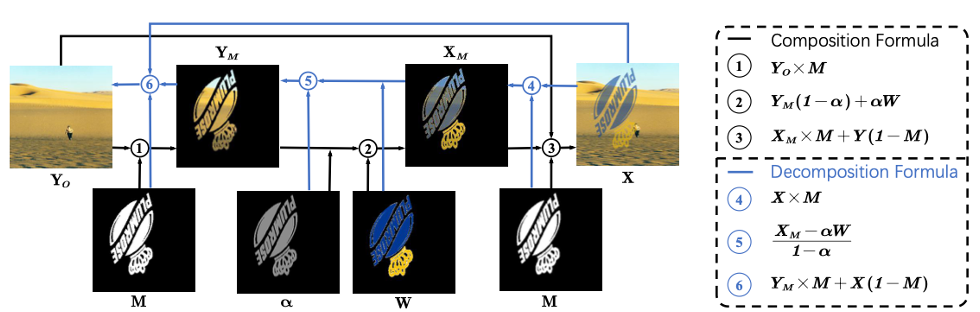
\includegraphics[width=\columnwidth]{29.png}
	\caption{水印嵌入过程和反过程示意图}
	\label{fig:29}
\end{figure}

受上述分析的驱动,Liu等~\cite{liu2021wdnet}拟在神经网络的生成器中构建水印图像的组合机制,其设计的WDNet具有深度学习方法从大规模数据集中学习的巨大能力,又兼具传统方法将水印与输入图像分离的能力。WDNet与先前的方法之间一个显著的区别是WDNet采用了两阶段的改进策略。Liu等认为水印去除任务隐含了一个预处理步骤——水印区域定位,这在先前的方法中被忽略了。因此,在WDNet的设计中显式地建模了这一过程,使得WDNet自然成为一个两阶段的生成器。

在第一阶段,WDNet不是直接估计无水印图像,而是通过预测粗糙的水印及其透明度来估计水印的大致区域,即($\hat{\alpha}, \hat{W}, \hat{M}$)。然后,根据网络估计的先验信息及水印嵌入的逆过程可以获得初步的无水印图像。然而,这一初步的结果并不令人满意,因为($\hat{\alpha}, \hat{W}, \hat{M}$)的值可能相互冲突,导致结果不够平滑。此外,这个结果仅粗略地表示了水印区域,需要进一步的细化。因此,在获得初始分解的无水印图像后,WDNet的第二阶段旨在通过从输出中获得额外的监督来对这些图像进行优化。由于第二阶段要求网络集中在像素级的细化上,而不是大范围和冗余的上下文,故此使用一个非常小的网络作为第二阶段的优化网络。具体来讲,它由几个残差块组成,有助于保证局部细化和高效性。和之前的工作类似,WDNet在第一阶段采用了U-Net的网络结构,并采用了基于补丁的鉴别器进行对抗训练。此外,WDNet不需要任何后处理过程。

\begin{figure}[!htbp]
	\centering
	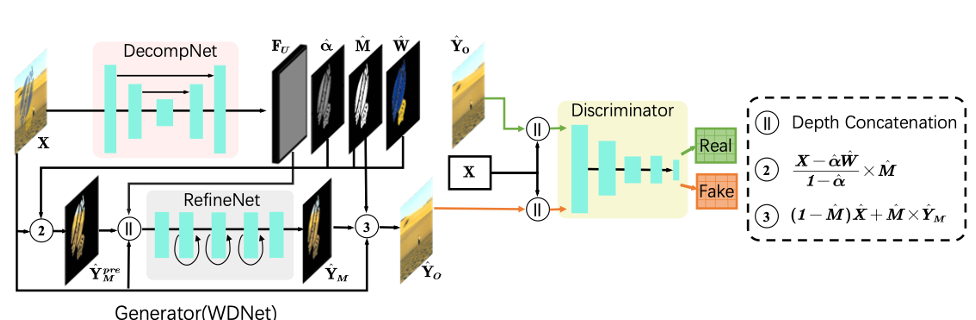
\includegraphics[width=\columnwidth]{30.png}
	\caption{WDNet架构图}
	\label{fig:30}
\end{figure}

\subsection{构建高效的水印去除模型}

在先前的工作中,检测水印位置是去除水印的前提,在获得水印嵌入位置后,可以通过图像修复或特征匹配来去除水印。Hertz等首次使用多任务网络来“盲”地从单幅图像中去除水印。然而,Liu等认为显示地学习水印嵌入区域是必要的。这种两阶段框架的基本思想是在多任务学习的架构下,由于嵌入水印图案与载体图像的纹理不协调,水印去除比检测更加复杂,因而需要对初步估计的原始图像进一步细化。如果背景(b)、预测掩码(e)和水印(g)由同一个网络生成,则背景(b)的视觉质量较差。其原因是因为水印去除需要从退化区域恢复确切的像素值,而水印检测只需要获取二进制掩码。因此,尽管可以像Hertz等那样使用单个多任务网络进行水印去除,但仍然需要使用预测的掩码(e)通过另一个网络对水印区域进行优化。基于上述分析,Cun等~\cite{cun2021split}提出了注意力引导的两阶段框架SplitNet和RefineNet。

\begin{figure}[!htbp]
	\centering
	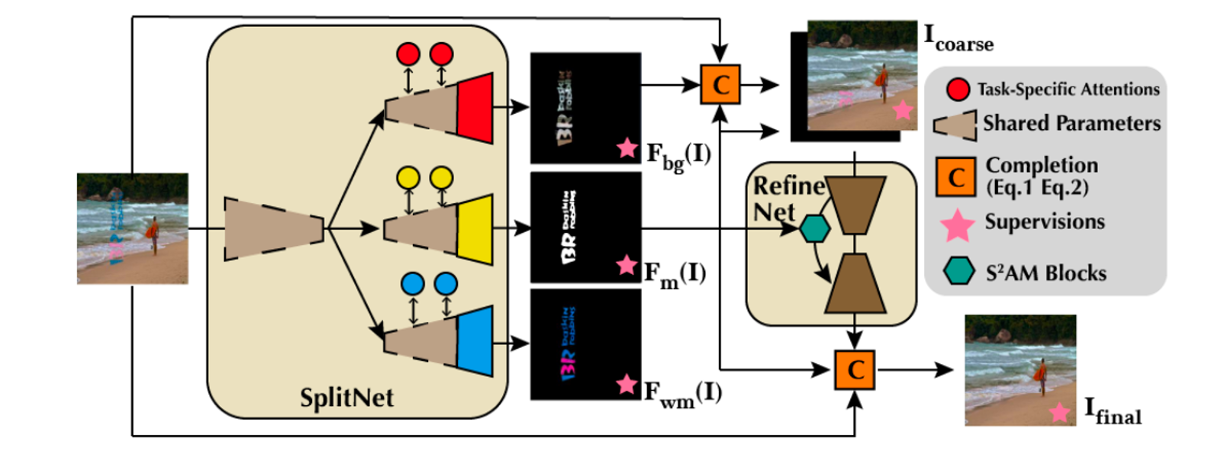
\includegraphics[width=\columnwidth]{31.png}
	\caption{两阶段网络架构图}
	\label{fig:31}
\end{figure}

在第一阶段,SplitNet使用基于残差块的U-Net作为基本的编码器-解码器结构,通过一个共享的编码器和多个解码器同时预测水印、背景和掩码,联合学习多个相关目标可以提升单个任务的性能。同时,将联合学习框架视为多域学习问题。在多域学习中,尽管每个域需要使用不同的参数,但为了学习一个高效的模型,几乎所有网络参数在训练过程中都是共享的。类似地,SplitNet中的三个任务在专注于学习一个空间区域的同时,每个任务都必须学习其重建任务相关的特定特征。具体而言,SplitNet三个解码器共享参数,并通过单独的域注意力学习每个任务的特定特征。这种策略有助于构建更高效和有效的模型。

在第二阶段,RefineNet,使用预测的掩码和SplitNet中的粗略结果进一步细化掩码区域像素。如果直接将掩码和粗糙结果作为第二阶段的输入,那么简单的网络可能无法专注于学习水印区域。因此,受空间分离注意力模块(S2AM)在图像和谐化中应用的启发,通过引入基于注意力的网络来改进预测的掩码区域。

\subsection{高质量掩膜预测的水印去除网络}

现有的水印去除方法可以分为两大类:(1) 端到端的全图擦除;(2) 同时检测水印和修复背景。第一种方法将水印去除的任务视为一个图像翻译的任务,即将带有水印的图片作为源域,无水印的图片作为目标域,通过近些年流行的图像翻译模型,实现水印擦除的功能,然而这样的方法只是隐式地告知模型水印的区域,很容易使得模型误擦除物体。第二种方法则是一种多任务的学习框架,同时执行水印检测与图像修复的任务,这样一来,在最后的图片修复中,模型只需要修复检测出来的水印区域,大大减小了误擦除的可能性。

对于前者而言,水印掩膜对于最终的图像修复质量非常重要,然而现有方法都没有针对水印检测做出优化。在实际应用中,水印的主体图案很容易被模型检测出来,然而水印周边的附属文字或者图案却很容易被模型视为噪声而忽视,这样检测出来的水印质量较差,而且会降低后续的修复的图像质量。

\begin{figure}[!htbp]
	\centering
	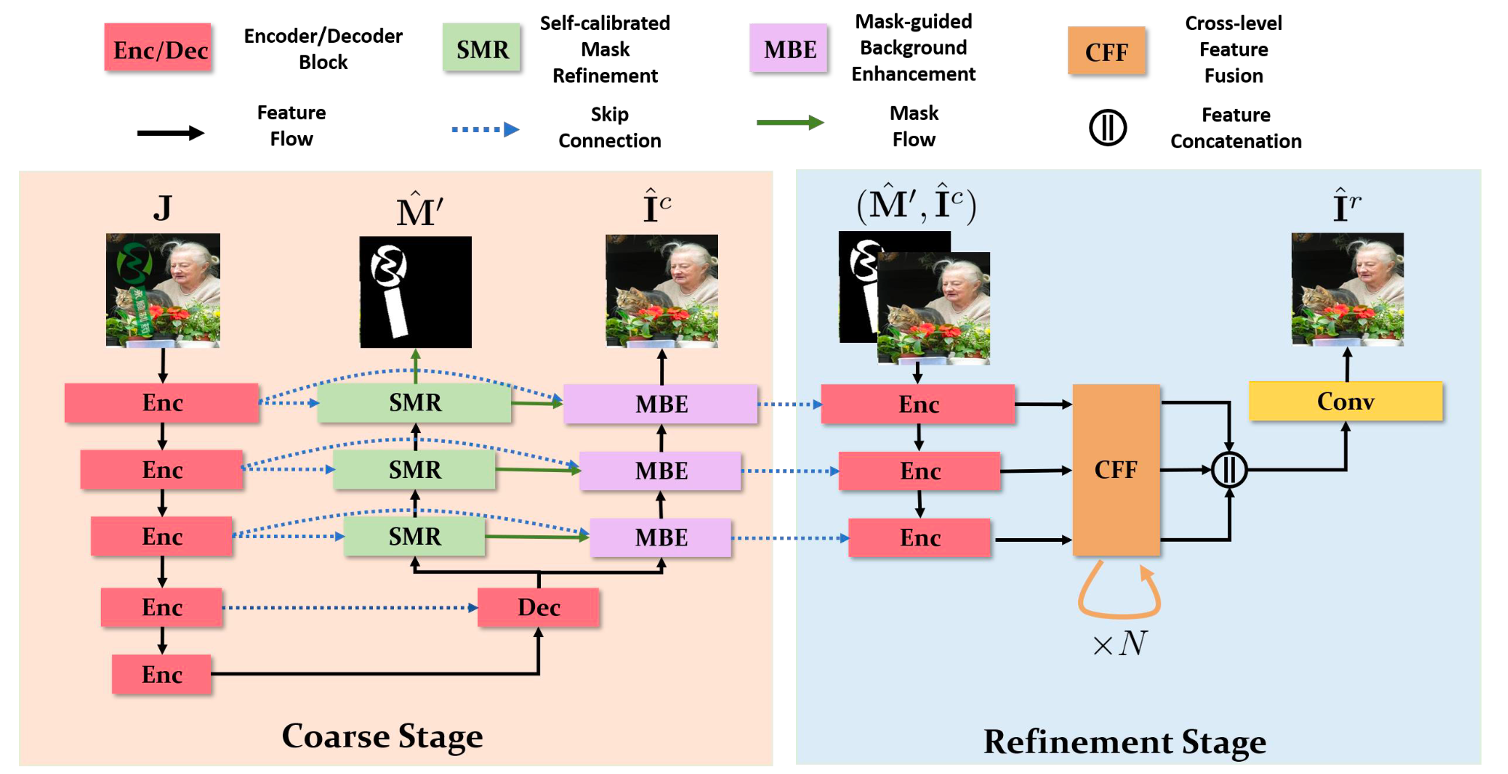
\includegraphics[width=\columnwidth]{32.png}
	\caption{基于自纠正水印检测模块和掩膜指引背景修复模块的可见水印去除网络架构图}
	\label{fig:32}
\end{figure}


为此,Liang等~\cite{liang2021visible}提出了自纠正的水印检测模块(Self-calibrated Mask Refinement),掩膜指引的背景修复模块,多层次信息融合的背景改进模块。整体框架可以分为背景粗修阶段,以及背景精修阶段。在背景粗修阶段,将水印定位和水印去除作为多任务学习框架中的两个任务。具体来说,网络由传统的U-Net结构演变而来,为了兼顾模型大小以及多任务的需求,采用了共享编码器以及一层共享解码器的主干网络,对于水印掩膜检测以及背景修复任务,则采用了不同的解码器分支实现不同的功能。掩膜解码器分支预测多尺度水印掩膜,通过掩膜引导的背景增强(MBE)模块为背景解码器分支提供指导,以更好地重建无水印图像。考虑到不同图像中的水印在许多方面存在很大的差异,设计了一个自校准掩膜细化(SMR)模块,将水印特征传播到整个特征图中,以更好地处理特定于图像的水印。在背景精修阶段,以预测的水印掩膜和粗度阶段的无水印图像作为输入,生成一个细化的无水印图像。为了充分利用粗修阶段的有用信息,在粗修阶段的背景解码器分支和细化阶段的编码器之间添加了跳连接。考虑到不同层次的特征捕获了结构信息或纹理细节,在精修阶段反复使用跨层次特征融合(CFF)模块来聚合多层次编码器特征。从精修阶段得到的输出图像是最终恢复的背景图像。

\begin{figure}[!htbp]
	\centering
	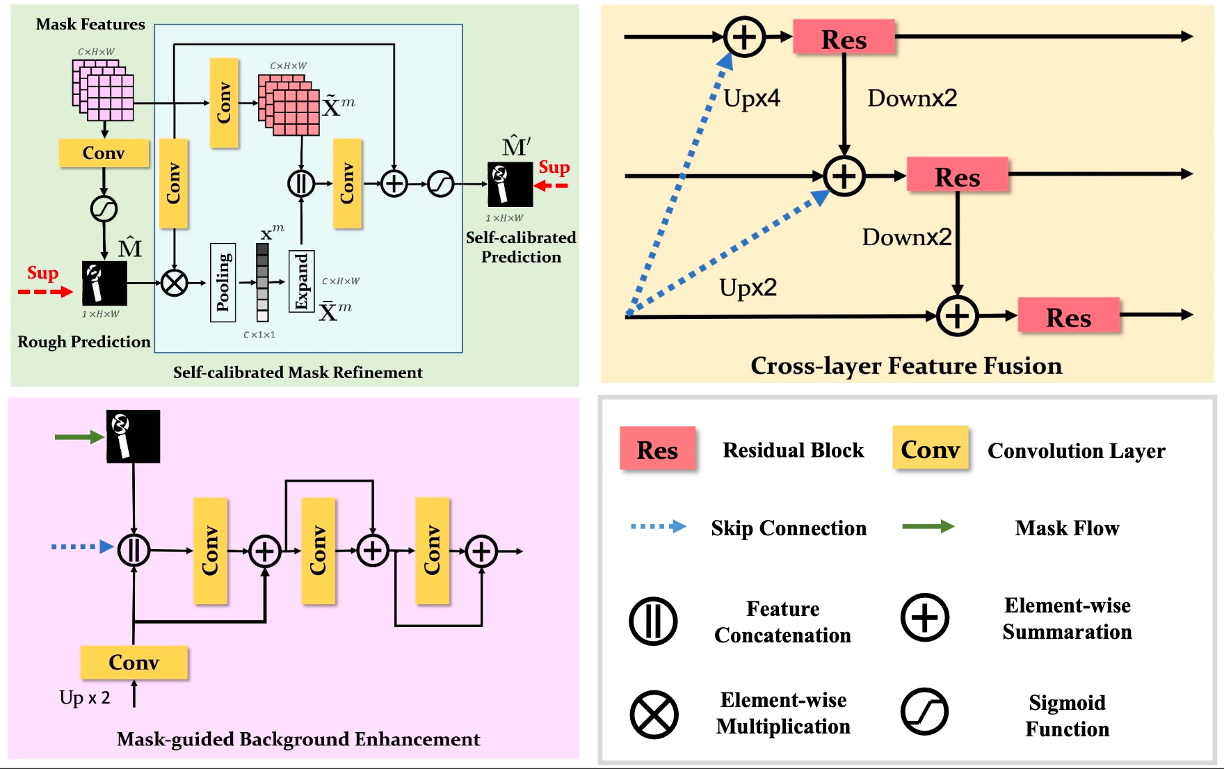
\includegraphics[width=\columnwidth]{33.png}
	\caption{自纠正的水印检测模块,掩膜指引的背景修复模块和多层次信息融合的背景改进模块示意图}
	\label{fig:33}
\end{figure}


自纠正水印检测模块分为两个部分,一个是常规的水印检测部分($X^m$以及$\hat{M}$),另一部分则是纠正掩膜的部分。在自纠正部分,作者希望学习到水印主图案的特征,将其在隐空间的特征与水印掩膜其他位置特征做相似度匹配,以此找出可能的环绕图案。在纠正模块中,首先从预测得到的水印掩膜的置信度图中,取出高置信度的掩膜,这一区域可以被认为代表了水印主体图案,随后将高置信度的掩膜与掩膜特征做点乘,并求平均得到一个均值向量$x^m$, 该向量可以表示为水印掩膜的主要特征;然而环绕在主图案的水印外表特征可能与主图案不一致,因此将水印掩膜主特征$x^m$投影到一个隐空间,得到$\bar{X}^m$,同时将水印特征也投影到隐空间,得到$\tilde{X}^m$,在此隐空间里将两个投影特征级联,通过1x1的卷积,即一个变换矩阵,学习相似度,最后得到了一个相似度图,在此相似度图里,只考虑正相关部分,因此可以使用水印掩膜标注作为监督,如此,可以识别出一些漏检并消除一些误报。

水印掩膜指引修复模块引入了预测的掩膜图作为指导。在跨层次特征融合中,考虑到分辨率较小的深层特征能够融合更多的语义信息,因此将其作为自下而上传播的特征流,在此结构中,可以看到信息可以自上而下以及自下而上的流动,充分地融合了背景修复的信息。

\begin{figure}[!htbp]
	\centering
	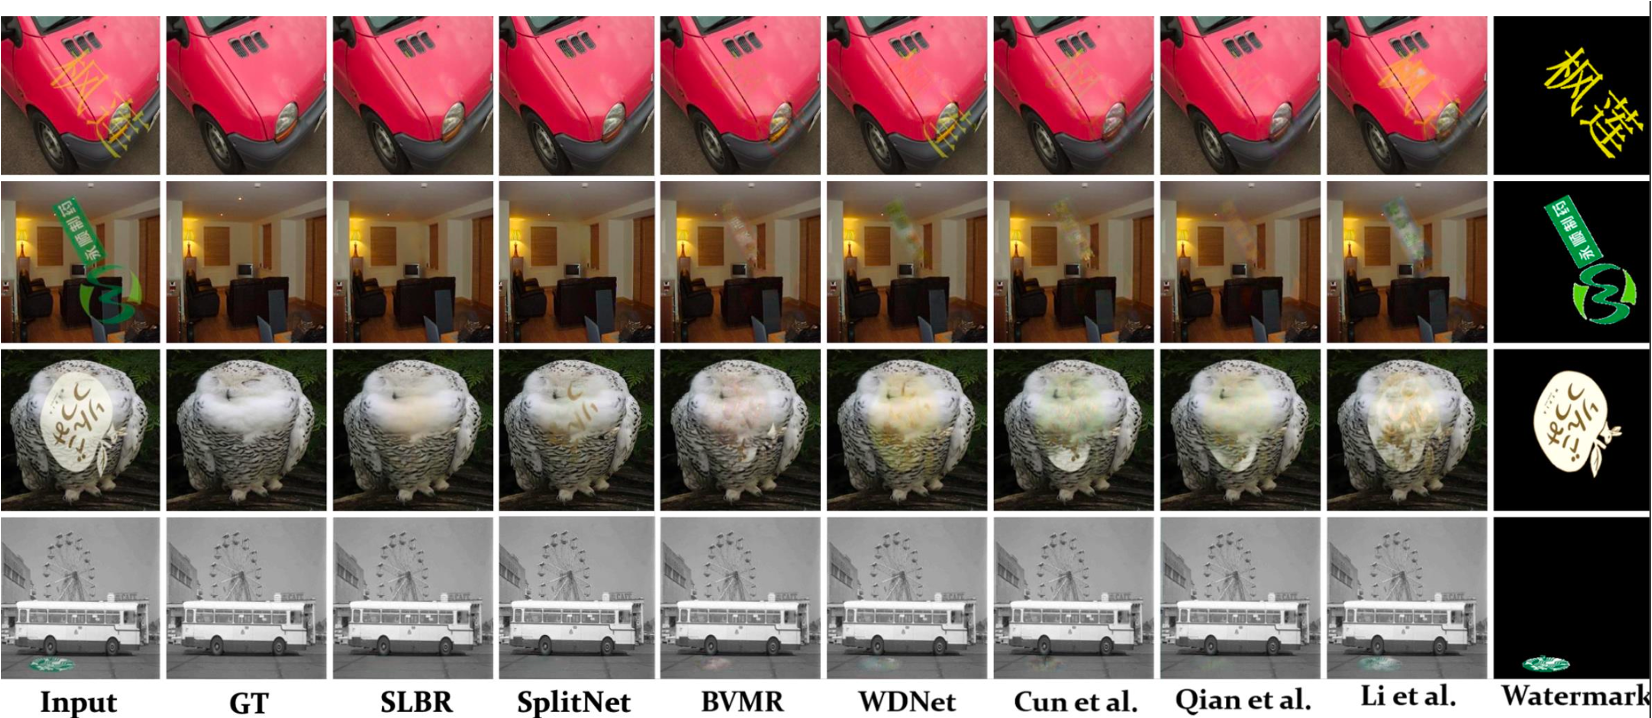
\includegraphics[width=\columnwidth]{34.png}
	\caption{水印去除结果示例图}
	\label{fig:34}
\end{figure}
\section{通用场景的图像视频修复}
\label{sec:other}

\subsection{光流引导的端到端视频修复}

针对水印去除的图像视频修复工作相对较少,更多的是通用的图像视频修复任务,过去的工作也多有采用图像视频修复方法作为水印去除的主要技术手段或细化方法。之前的视频补全方法,大致可以分为三类:第一类为非深度学习时代的Patch-borrowing的方法,这类方法先根据输入视频或外部数据建立一个volume,每个待补全的图像块都会在这个volume中寻找相似的图像块来更新待补全的区域。第二类为深度学习时代中基于autoencoder的方法,这类方法主要依托于类U-Net的网络结构,这其中会引入比如说3d convolution、gated convolution或是在bottleneck的地方使用transformer来进行端到端的视频补全。第三类为基于光流的方法。

基于光流的方法将视频补全看作是像素传播的过程,其主要包含了三个阶段,第一阶段为光流补全,由于mask掉的区域光流是无法直接估计的,所以就需要借助mask外区域的光流来对缺失的部分进行补全。光流由于其结构和纹理都相比视频简单,所以光流补全要比视频补全容易得多。第二阶段为像素传播,借助补全后的双向光流来索引邻近帧中对应的像素对缺失部分补全。第三步为内容幻化,对于传播过程中没有索引到的区域,通过一个预训练的图像补全网络来完成最后的填充。这三个阶段是分别执行的,并不是端到端的,这样一个视频补全系统存在许多缺点:由于第一个阶段与第二个阶段存在许多复杂的手工设计的操作,因此计算效率很低,处理70帧的不到360p的视频就需要约4分钟。同时由于这三个阶段是分别执行的,每个阶段都非常依赖上个阶段的生成的结果,因此容易造成误差的累积与放大。最后一阶段所使用图像补全网络只考虑了单帧信息,因此生成的结果时间及空间的一致性不是很高。

为解决上述问题,Li等~\cite{li2022towards}希望模拟之前基于光流引导的方法的三个阶段,去设计对应的三个模块,以构建一个可以被端到端优化的视频补全框架。首先,将像素传播过程转换为了通过光流引导的特征传播过程。其次将负责光流补全的网络嵌入整个网络框架中,通过额外的光流补全损失使其与其他网络模块一同被端到端地优化。最后在内容幻化模块中,使用temporal focal transformer同时融合局部邻域与非局部视频帧的信息。

\begin{figure*}[!htbp]
	\centering
	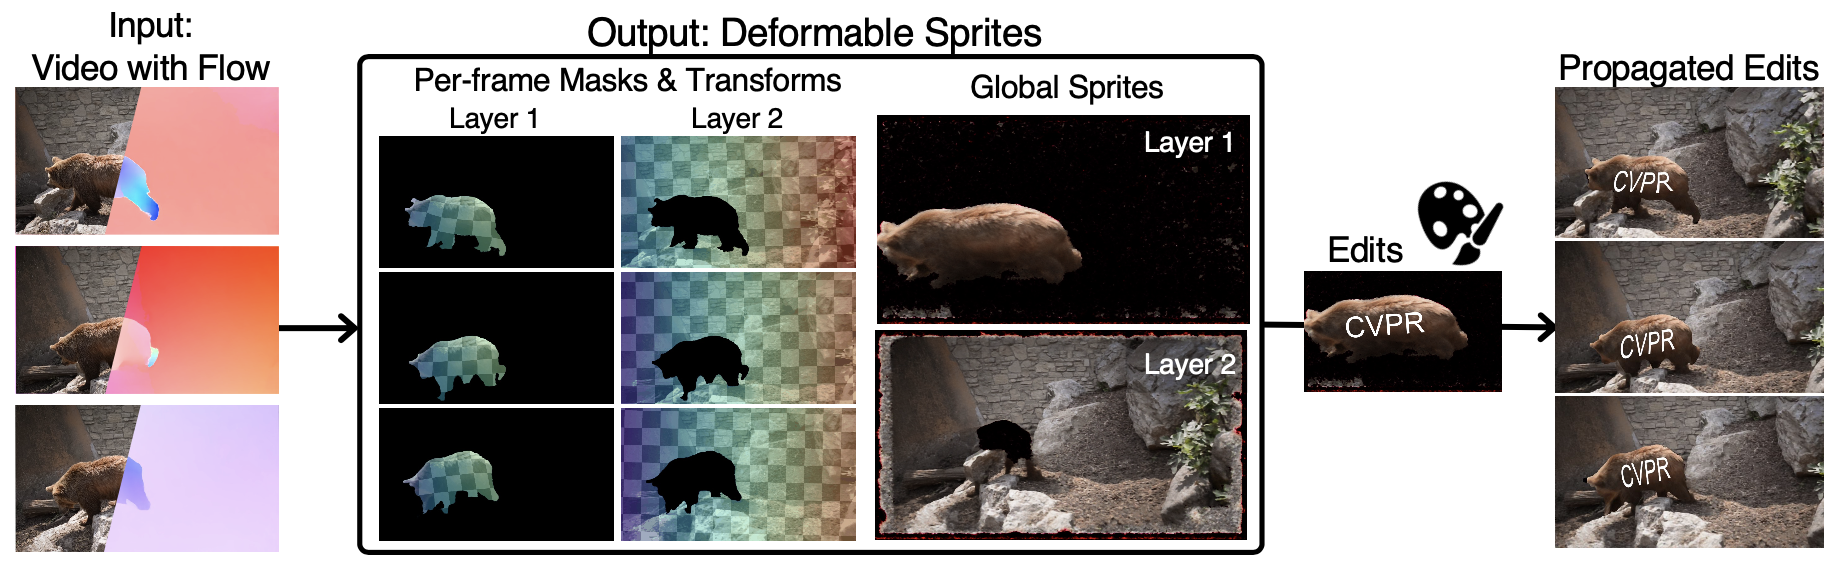
\includegraphics[width=\linewidth]{37.png}
	\caption{光流引导的端到端视频修复网络架构图}
	\label{fig:37}
\end{figure*}

\begin{figure}[!htbp]
	\centering
	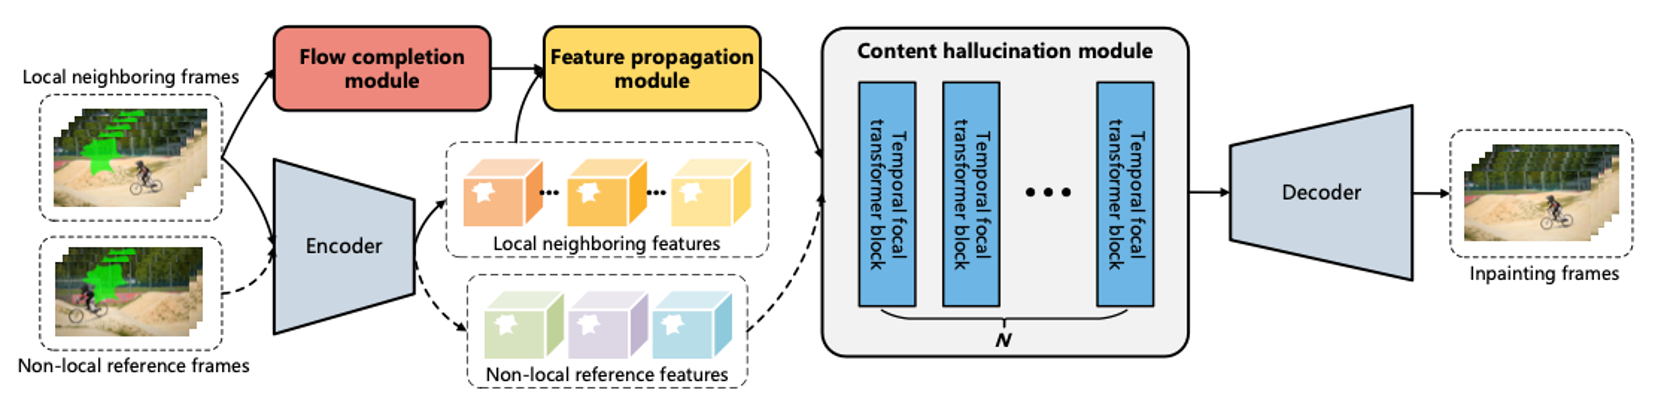
\includegraphics[width=\columnwidth]{35.png}
	\caption{光流引导的端到端视频修复网络架构图}
	\label{fig:35}
\end{figure}

为了实现端到端的光流补全,首先将一个用于光流估计的网络嵌入整个网络框架中作为光流补全模块,并使用额外的光流补全损失来监督。通过这一监督,可以让该光流补全模块同时完成光流的估计与补全。简单起见,我们使用L1 loss来对光流补全模块输出的双向光流进行监督。整个围绕光流补全模块的设计有两点优势:一是该损失可以配合网络其他任务导向的损失一同约束该模块的优化,让这一模块生成任务导向的光流。二是仅需要一个光流估计的子网络就可以直接进行光流的补全,整个光流补全的过程也相较之前的方法更加高效,大约可以快出40倍。

\begin{figure}[!htbp]
	\centering
	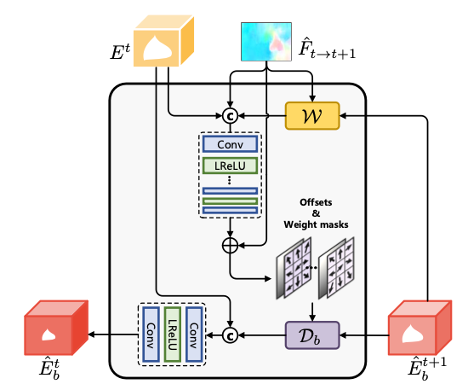
\includegraphics[width=0.9\columnwidth]{36.png}
	\caption{光流引导的可变性卷积结构图}
	\label{fig:35}
\end{figure}

得到补全的光流后,可以将邻近帧的特征根据光流进行索引并warp,进而实现特征的传播。但由于补全后的光流肯定没办法做到100\%准确,不准确的光流信息会导致在特征传播过程中引入无关的信息,进而影响最终的结果。为此,引入deformable convolution来补救这些不好的光流补全结果。Deformable convolution可以让sample点的位置更多更灵活,同时自适应地汇聚这些信息,使特征传播过程更加有效。而光流可以为deformable convolution给出更好的起始sample点选择,使其更容易sample到有意义的内容信息。

在inpainting中为了补全缺失部分的信息,一种很朴素的想法就是全局暴力搜索相似图像块,但这样的方式计算复杂度高,计算效率很低。对于一块缺失区域而言,与其最相似的内容应该在其周围,越远的区域与其内容越不相似。之前也有一些image inpainting的工作,通过设计权重,在进行填充的时候,mask周围的区域权重大,离mask远的区域权重小。本文使用了focal attention,即在局部区域使用细粒度的attention,在全局使用粗粒度的attention。
\section{水印嵌入}
\label{sec:embed}

\subsection{视频水印嵌入}

如前文所述,水印去除作为一种攻击手段,可以为开发更加鲁棒的水印嵌入技术提供线索。Ye等~\cite{ye2022deformable}设计了从输入视频中提取动态场景中持久元素的方法,将每个场景元素表示为可变形的精灵(Deformable Sprite),由三部分组成:1)贯穿整个视频的2D纹理图像,2)元素的逐帧掩码,3)将纹理图像映射到每个视频帧的非刚性形变。得到的分解结果可以用于一致的视频编辑等应用,例如将水印根据纹理和形变动态地嵌入到视频中的对象,可以实现更好的嵌入效果,同时相较于静态水印给水印的去除带来更大的难度。

\subsection{扩散模型和水印}
可以看到,现有工作多依赖于GAN网络来恢复更加真实的水印去除图像,并取得了相当不错的性能表现。同样作为生成模型,扩散模型可以在相同任务上生成更加真实的图像。尽管尚未出现基于扩散模型的针对水印去除任务的研究,但通用的图像修复模型~\cite{yildirim2023inst,rombach2022high}已如雨后春笋般涌现,一般而言,这些模型也适用于水印去除的图像修复。

除此以外,以水印去除作为攻击手段,研究人员旨在借此设计更加鲁棒的水印嵌入方法。而以扩散模型为代表的生成模型在应用于各种领域的同时,也引发了关于负责任部署的道德关注。因此,将图像水印和扩散模型相结合,让所生成的图像嵌入不可见的水印,以便未来进行检测或识别\cite{fernandez2023stable},也已成为研究的热点。
\section{结论}
\label{sec:conclusion}

水印在日常生活中随处可见,它是一种保护图像视频版权的机制,防止未经许可或授权的使用。在很多的情况下,人们可能希望去除这些水印图像以获得不被遮盖的原始图像。然而,由于水印可以覆盖在各种大小、形状、颜色和透明度的背景图像上的任意位置,同时其通常包含复杂的图案,如扭曲的符号、细线、阴影效果,这使得去除这些水印图像并恢复原始图像是一项具有挑战性的任务。如果没有人工指导或关于载体图像的假设,将很难检测到水印图像并重建原始图像。近年来,随着计算机硬件的不断发展,计算机的计算能力也显著提高,从而推动了深度学习方法的快速进步并产生了一系列基于卷积神经网络的技术。从研究发展历程来看,水印去除既可以采取通用的目标检测模型和图像修复模型,又可以根据任务特性设计专门的模块和网络架构重建视觉效果更好图像。在过去,U-Net、GAN网络等模型架构在水印去除任务上一直作为主流的网络模型并取得了很好的性能表现。放眼未来,我们也期待有更多的研究可以基于现如今性能更加强大的网络设计(如 Transformer、扩散模型等)以实现更好的水印去除和图像视频修复效果。在这个繁荣的信息时代,水印去除技术的发展也在不断推进水印嵌入技术的进步,这对于网络信息安全领域具有重要意义。


% Can use something like this to put references on a page
% by themselves when using endfloat and the captionsoff option.
\ifCLASSOPTIONcaptionsoff
  \newpage
\fi



{\small
\bibliographystyle{IEEEtran}
\bibliography{reference/egbib}
}

% that's all folks
\end{sloppypar}
\end{document}


